% =================================================================================================
% File:			diagrammi attivita.tex
% Description:	Defiinisce la sezione relativa a ...
% Created:		2015-02-23
% Author:		Tesser Paolo
% Email:		tesser.paolo@mashup-unipd.it
% =================================================================================================
% Modification History:
% Version		Modifier Date		Change											Author
% 0.0.1 		2015-02-23 			sistemato header								Tesser Paolo
% =================================================================================================
% 0.0.2			2015-03-19			cambiata logica diagrammi e estesa				Tesser Paolo
% =================================================================================================
% 0.0.3			2015-03-19			stese le note principali per ogni diagramma		Tesser Paolo
% =================================================================================================
% 0.0.4			2015-03-22			inclusi diagrammi								Tesser Paolo
% =================================================================================================
% 0.0.5			2015-03-26			scritte descrizioni generali dei diagrammi		Tesser Paolo
% =================================================================================================
%

% CONTENUTO DEL CAPITOLO

\section{Diagrammi delle attività} % (fold)
\label{sec:diagrammi_delle_attivita}
In questa sezione vengono illustrati i diagrammi delle attività che descrivono le interazione dei diversi tipi di utente con il prodotto. Per ogni utente che interagisce con il sistema verrà rappresentato un diagramma principale delle attività che può svolgere, andando poi a raffinare le singole con ulteriori grafici maggiormente dettagliati. \newline
I diagrammi vengono classificati con il seguente formalismo:
	\begin{center}
		D[Codice]
	\end{center}
	\noindent
Dove [Codice] è un valore gerarchico.

	\subsection{Utente non autenticato} % (fold)
	\label{sub:utente_non_autenticato}
	In questa sezione vengono illustrate le attività che un utente non registrato o non ancora autenticato al sistema può compiere.
		\subsubsection{D1: Attività principali dell'utente non autenticato} % (fold)
		\label{ssub:attivita_principali_dell_utente_non_autenticato}
		\begin{figure}[!htbp]
			\centering
			\centerline{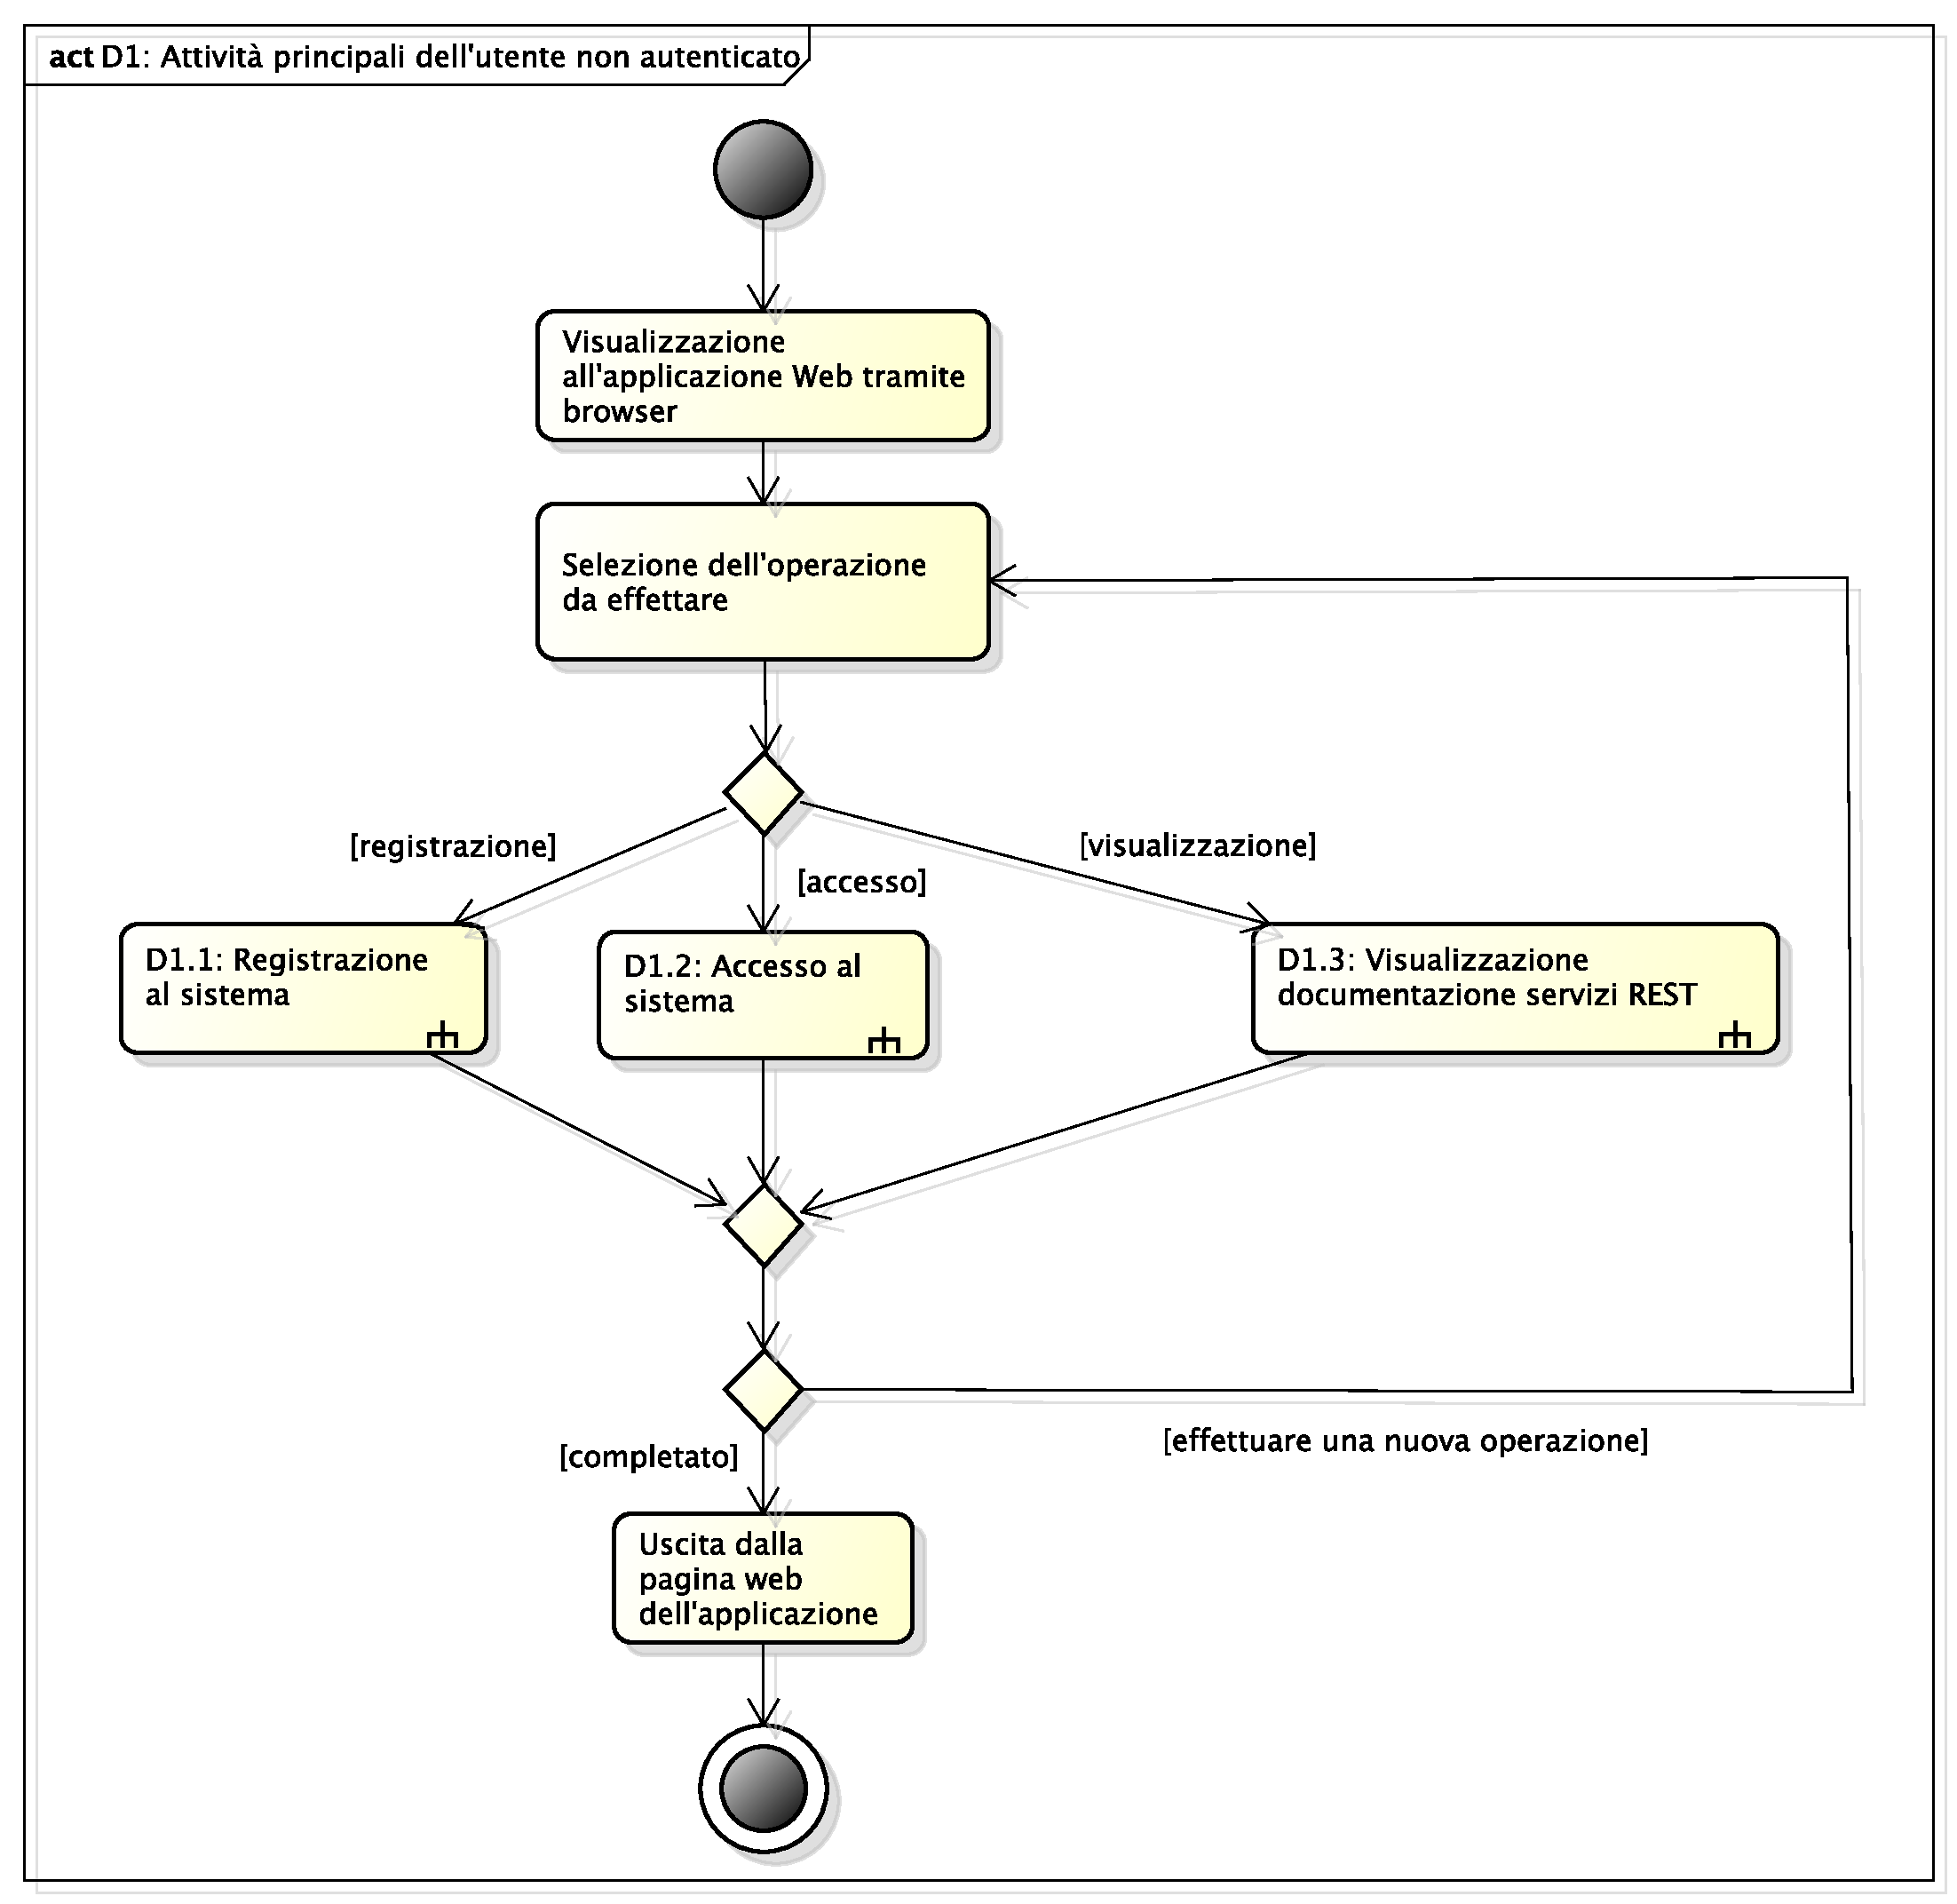
\includegraphics[scale=0.67]{./images/D1.pdf}}
			\caption{D1 - Diagramma delle attività principali dell'utente non autenticato}
		\end{figure}
		\noindent
		L'utente che entra nell'applicazione web ha la possibilità di registrarsi o di effettuare il login qualora fosse già registrato al sistema. Li viene inoltre offerta la possibilità di vedere la documentazione dei servizi REST che vengono offerti. Esso però potrà utilizzarli solo dopo essersi registrato ed avare fatto richiesta del token di accesso.

		% subsubsection attività_principali_dell_utente_non_autenticato (end)


		\subsubsection{D1.1: Registrazione al sistema} % (fold)
		\label{ssub:registrazione_al_sistema}
		\begin{figure}[!htbp]
			\centering
			\centerline{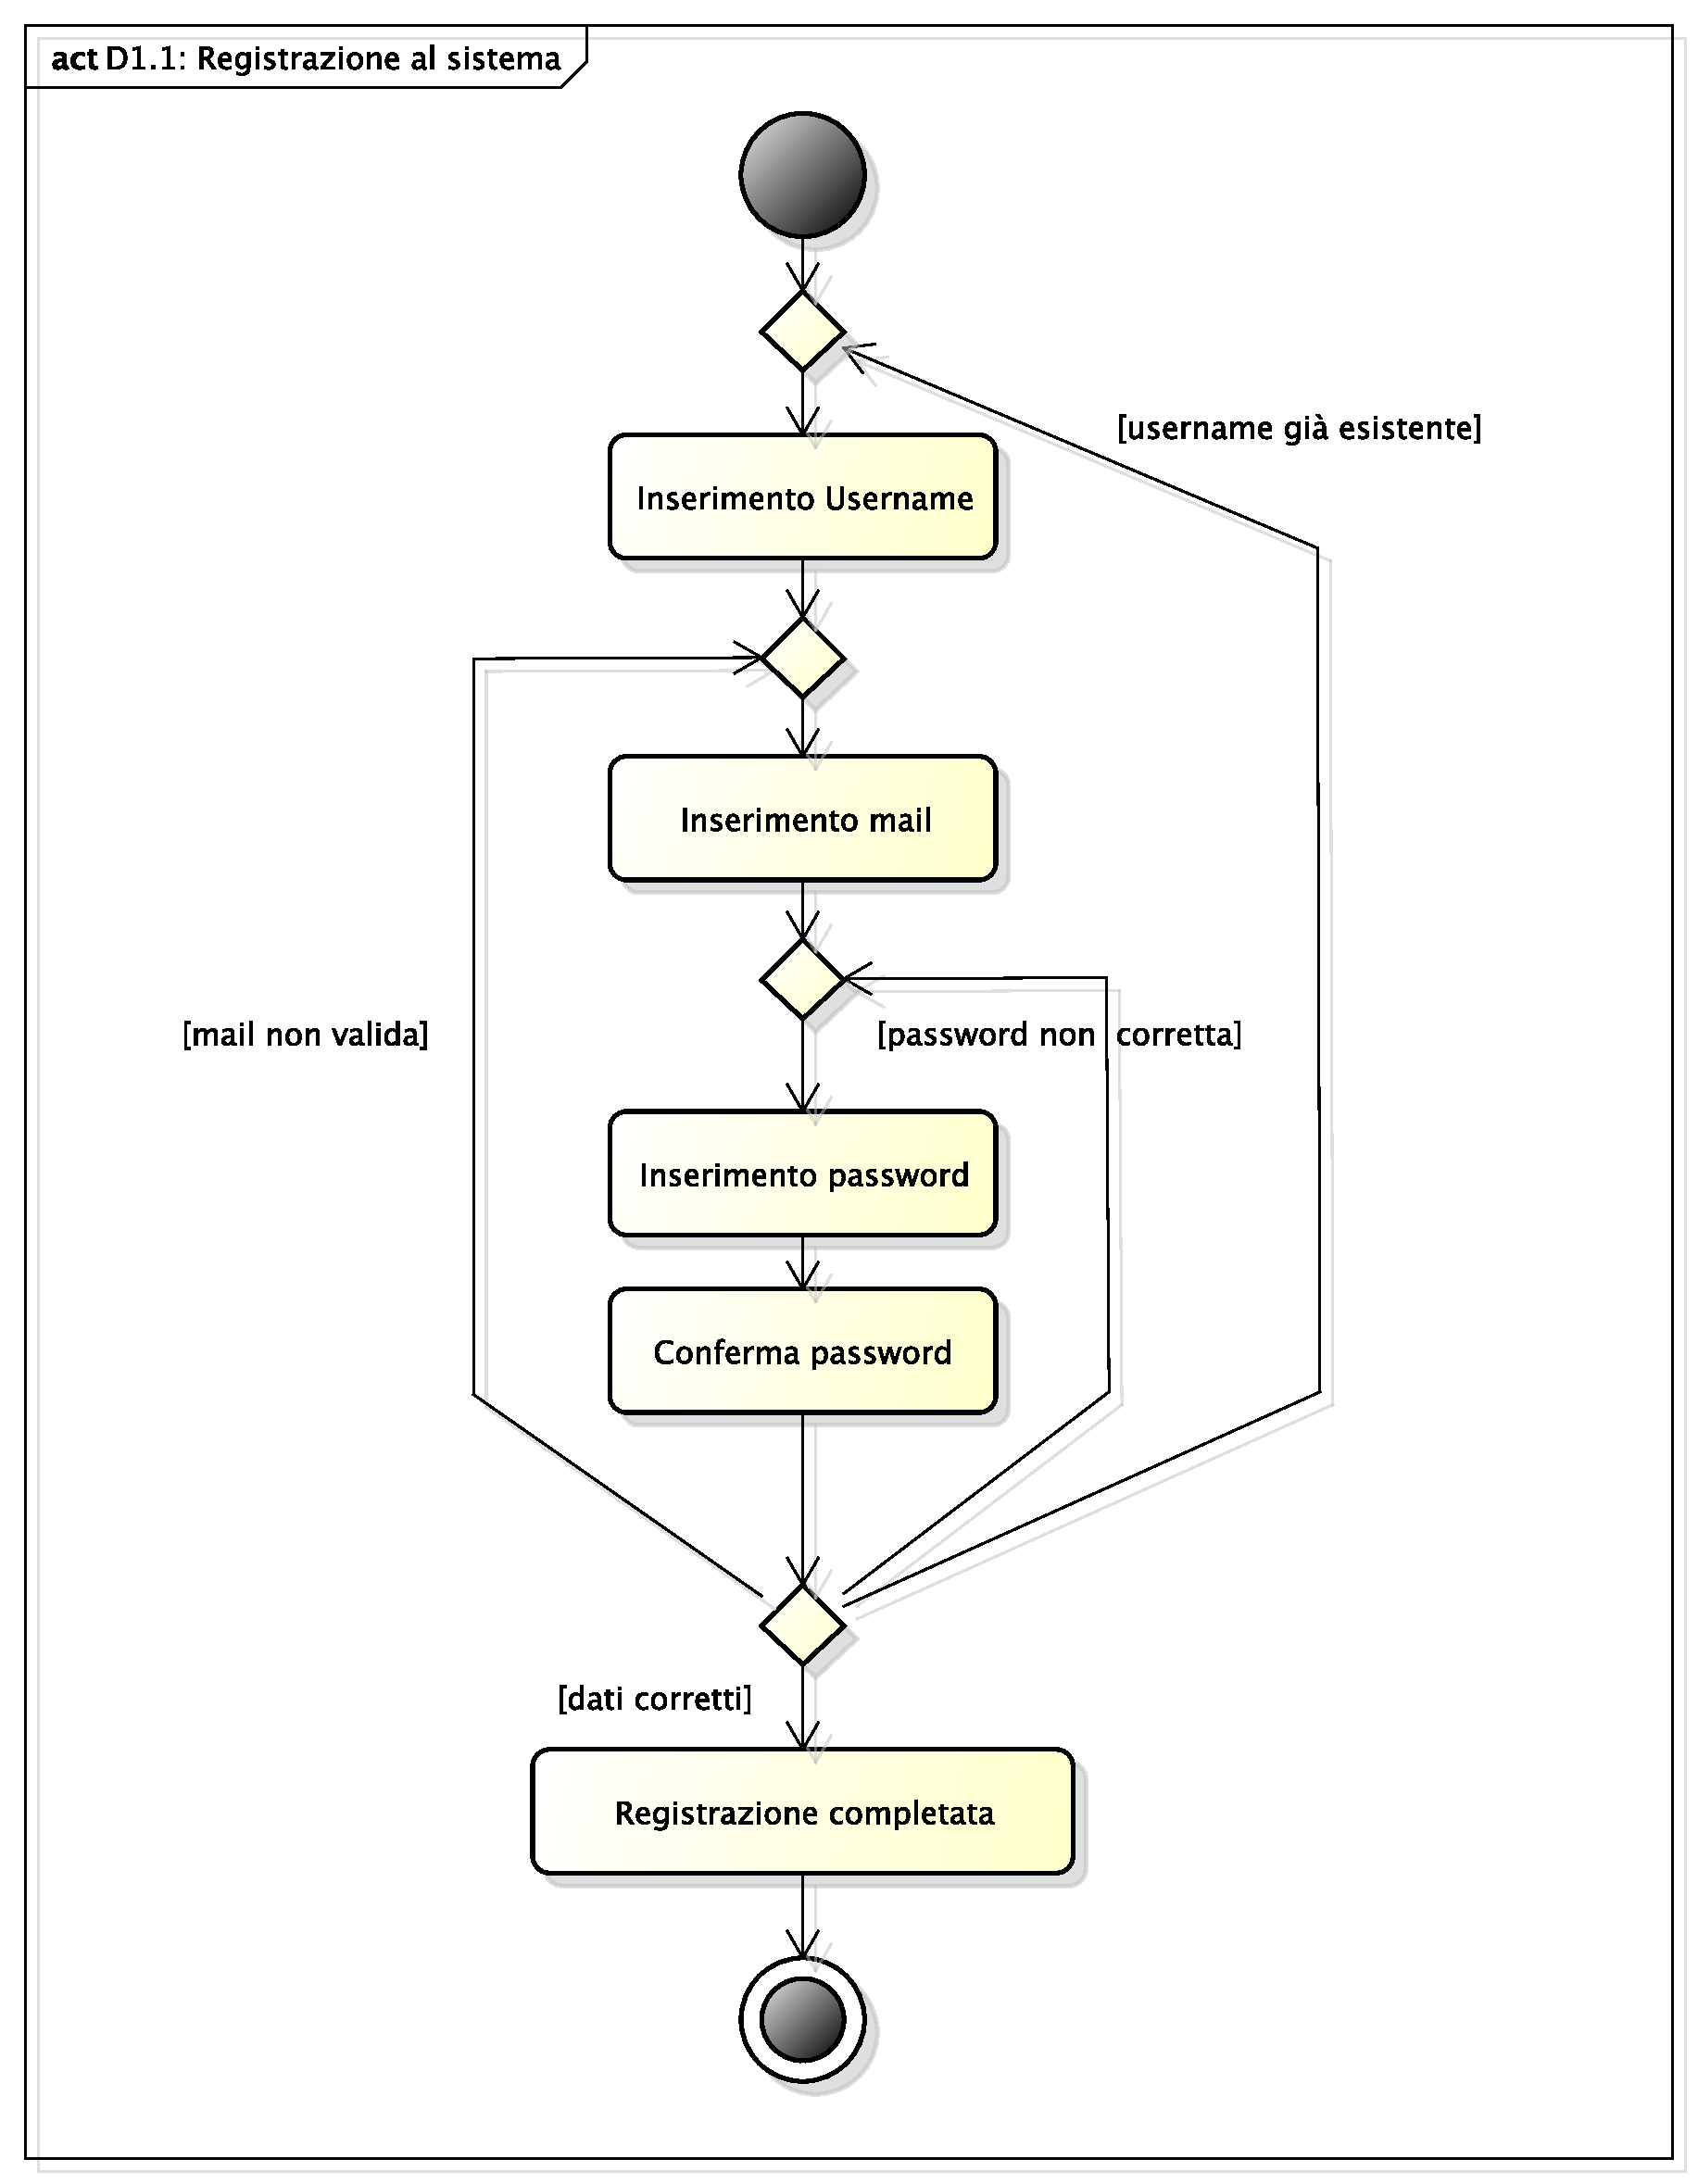
\includegraphics[scale=0.45]{./images/D1_1.pdf}}
			\caption{D1.1 - Diagramma della registrazione al sistema}
		\end{figure}
		\noindent
		Per registrarsi, l'utente dovrà inserire uno username, non già presente nel sistema, la mail e la password. Qualora tutti i dati inseriti fossero corretti, potrà confermare la registrazione e utilizzare i dati in seguito per accedere all'applicativo.
		% subsubsection registrazione_al_sistema (end)

		\pagebreak

		\subsubsection{D1.2: Accesso al sistema} % (fold)
		\label{ssub:accesso_al_sistema}
		\begin{figure}[!htbp]
			\centering
			\centerline{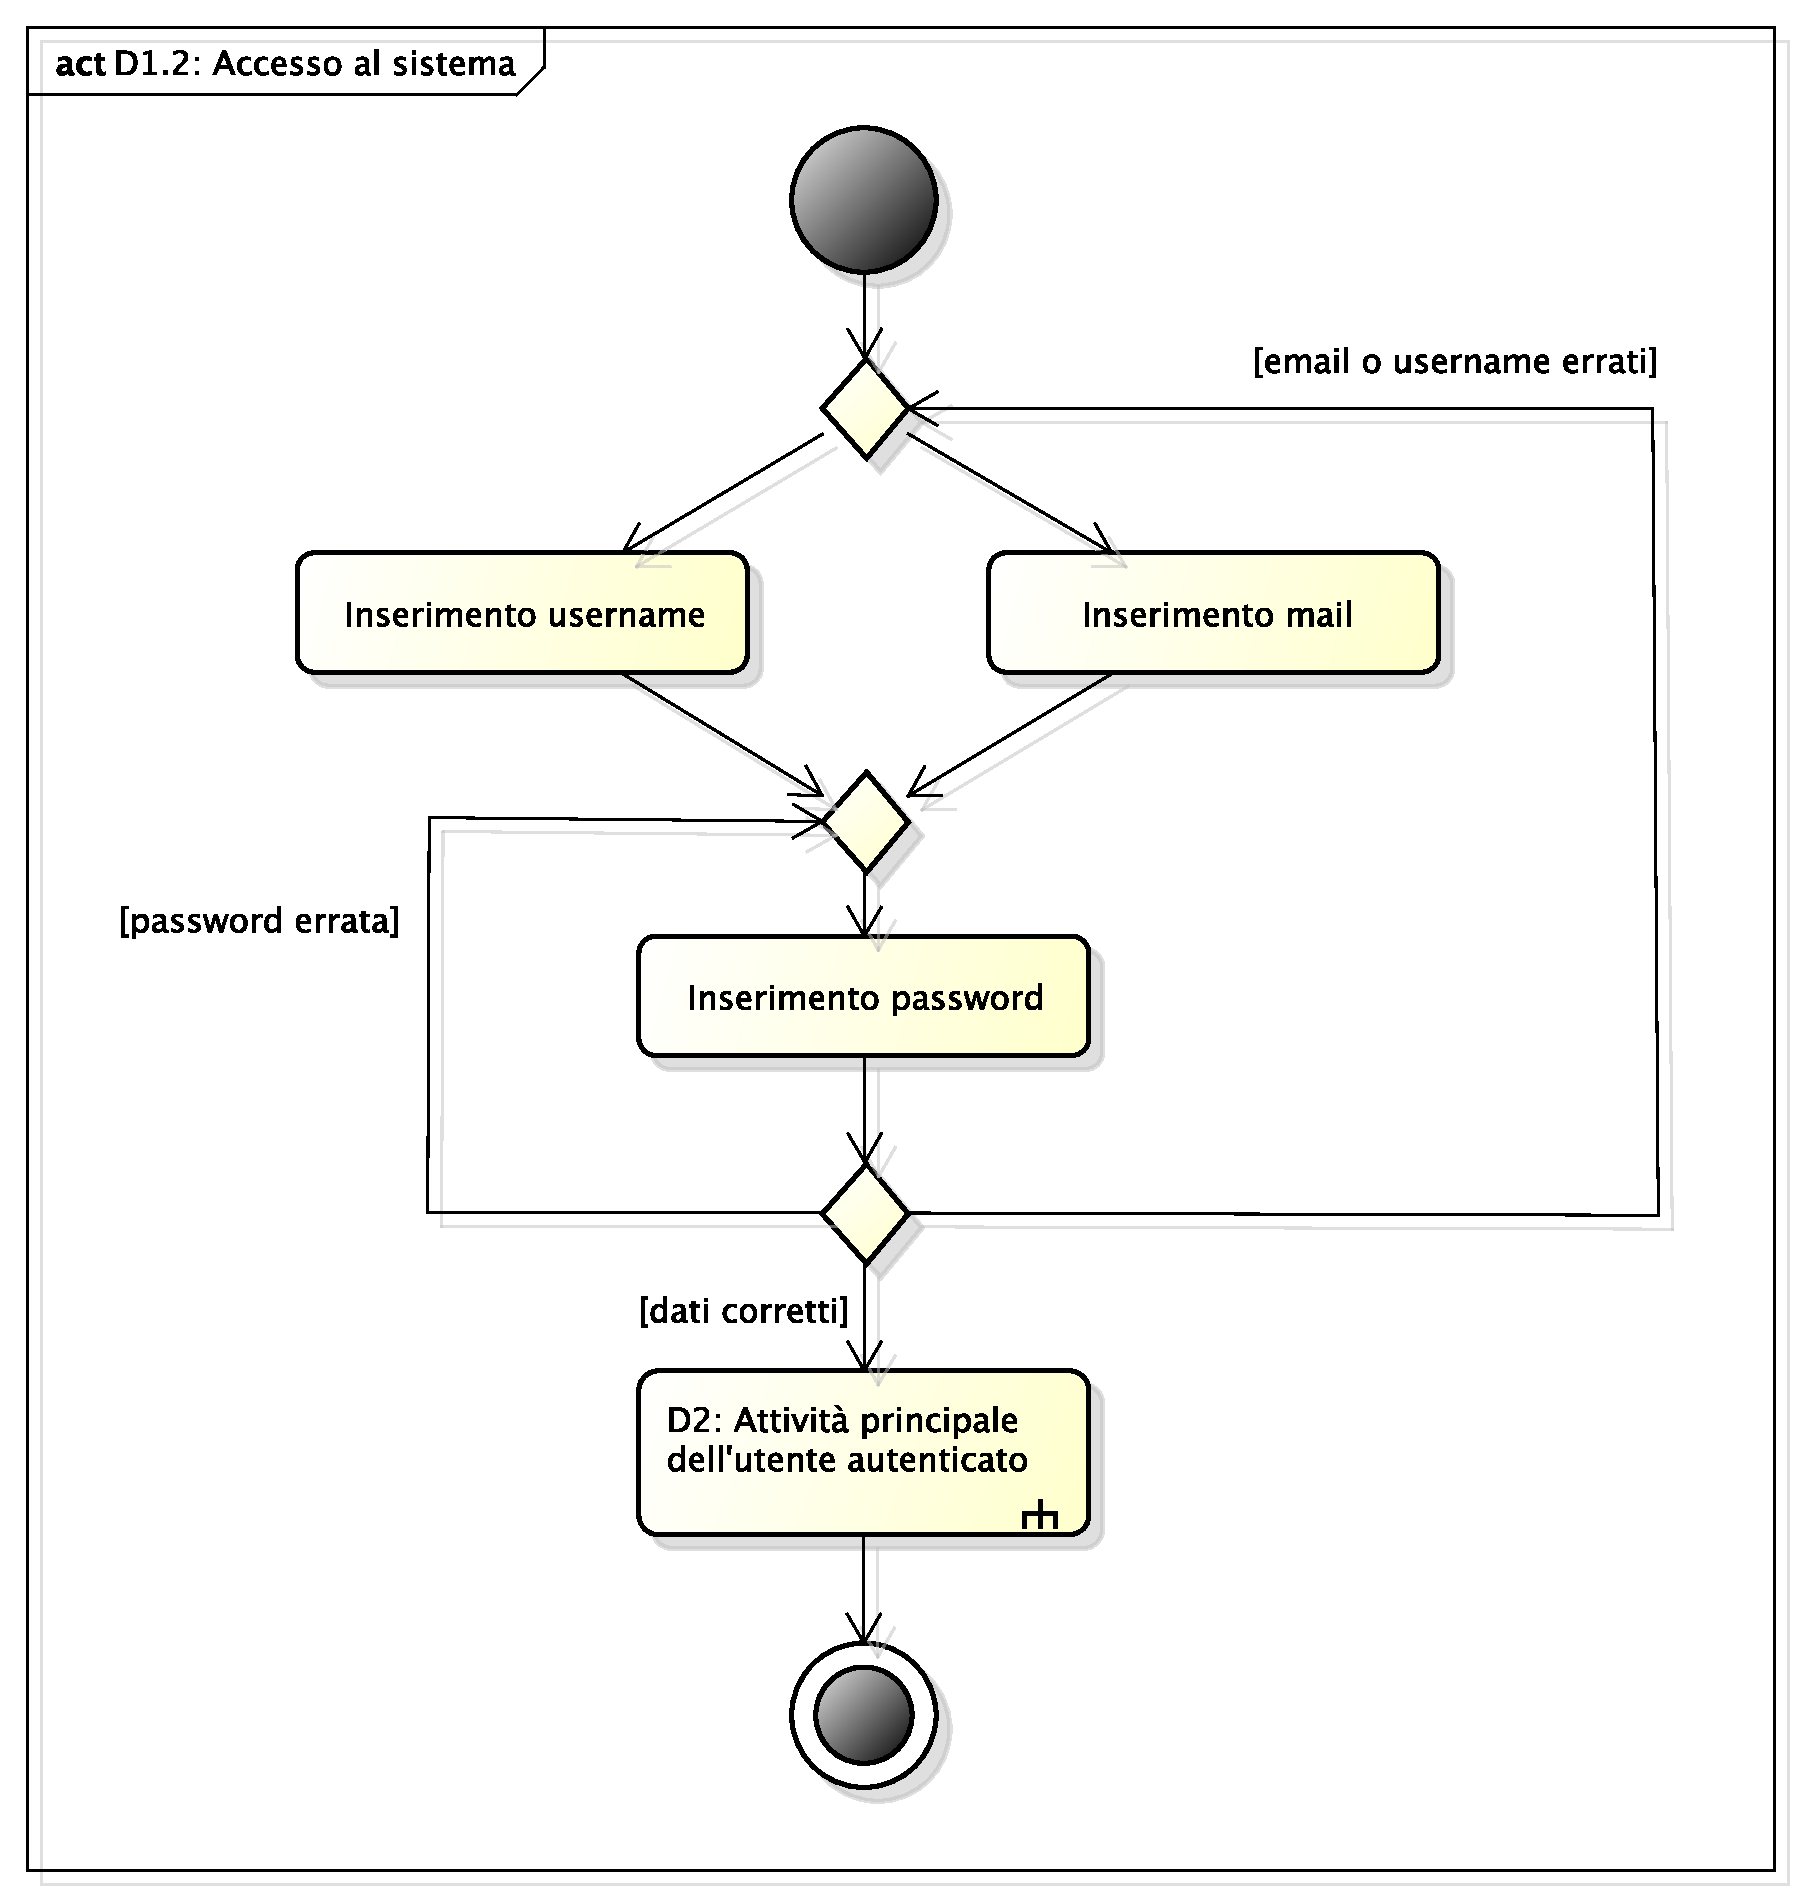
\includegraphics[scale=0.45]{./images/D1_2.pdf}}
			\caption{D1.2 - Diagramma dell'accesso al sistema}
		\end{figure}
		\noindent
		Per effettuare il login, l'utente dovrà inserire o lo username o l'email e inseguito la password d'accesso. Qualora tutti i dati inseriti fossero corretti, potrà accedere all'applicativo, altrimenti dovrà correggere gli errori segnalati. \newline

		% subsubsection accesso_al_sistema (end)

		\pagebreak

		\subsubsection{D1.3: Visualizzazione documentazione servizi REST} % (fold)
		\label{ssub:visualizzazione_documentazione_servizi_rest}
		\begin{figure}[!htbp]
			\centering
			\centerline{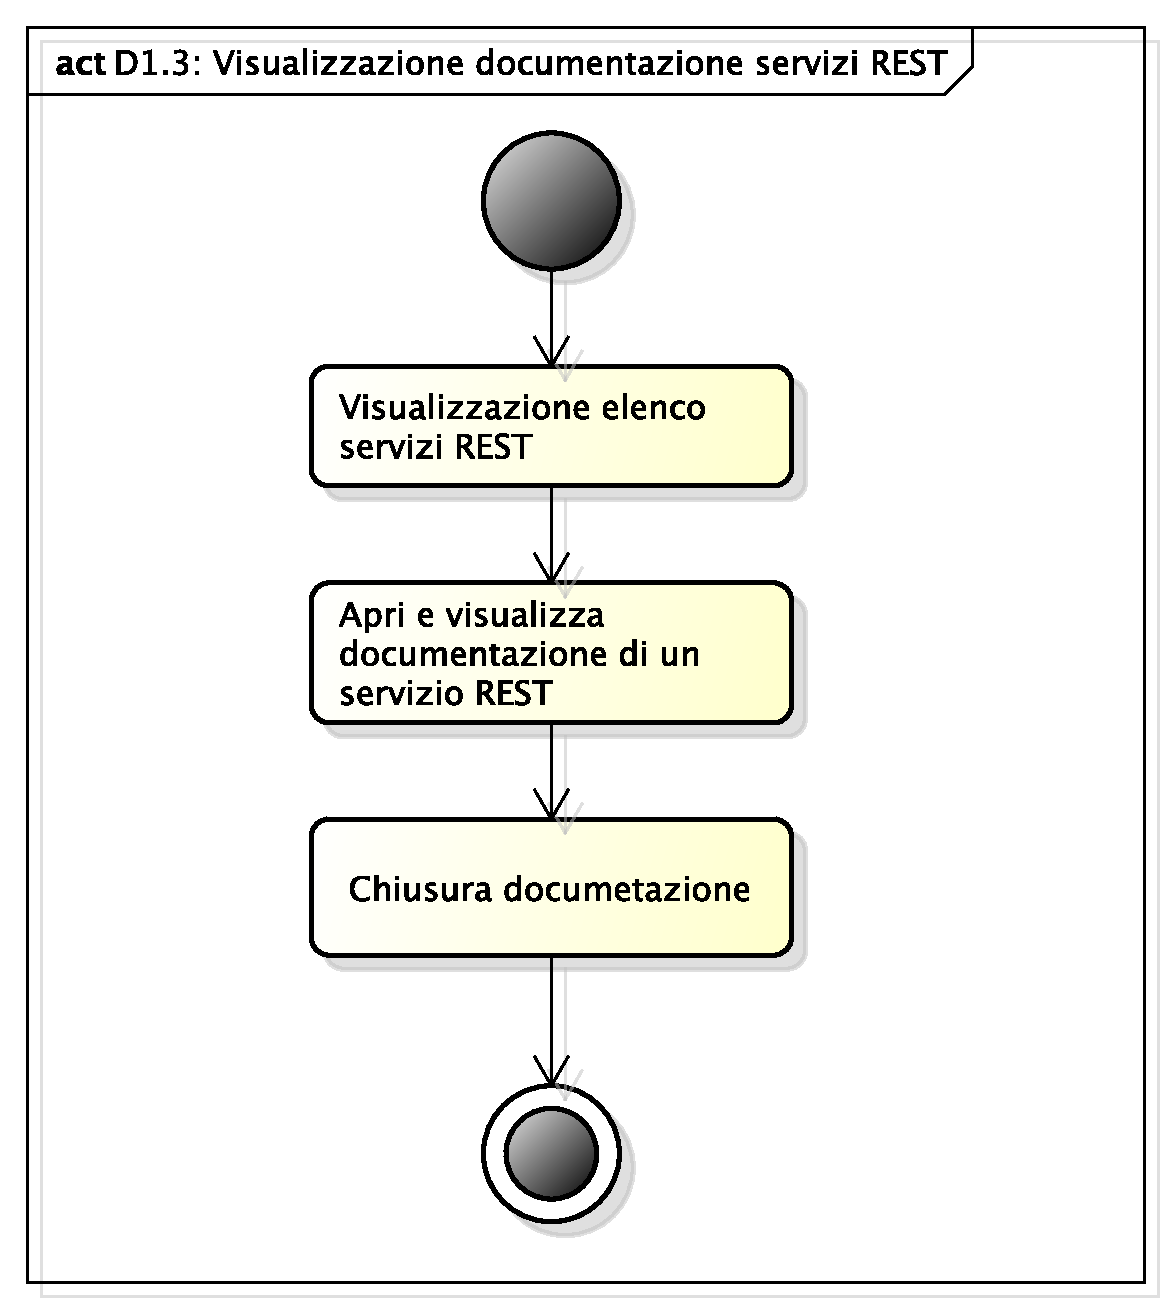
\includegraphics[scale=0.45]{./images/D1_3.pdf}}
			\caption{D1.3 - Diagramma della visualizzazione documentazione servizi REST}
		\end{figure}
		\noindent
		Anche all'utente non autenticato viene fornita l'opportunità di visualizzare la documentazione dei servizi REST che l'applicativo offre. Entrando su un particolare servizio potrà vedere nel dettaglio la specifica. Potrà utilizzarli solo però registrandosi all'applicativo.
		% subsubsection visualizzazione_documentazione_servizi_rest (end)

	% subsection utente_non_autenticato (end)

	\pagebreak
	\clearpage \newpage

	\subsection{Utente autenticato} % (fold)
	\label{sub:utente_autenticato}
	In questa sezione vengono illustrate le attività che un utente autenticato al sistema può compiere.
		\subsubsection{D2: Attività principali dell'utente autenticato} % (fold)
		\label{ssub:attivita_principali_dell_utente_autenticato}
		\begin{figure}[!htbp]
			\centering
			\centerline{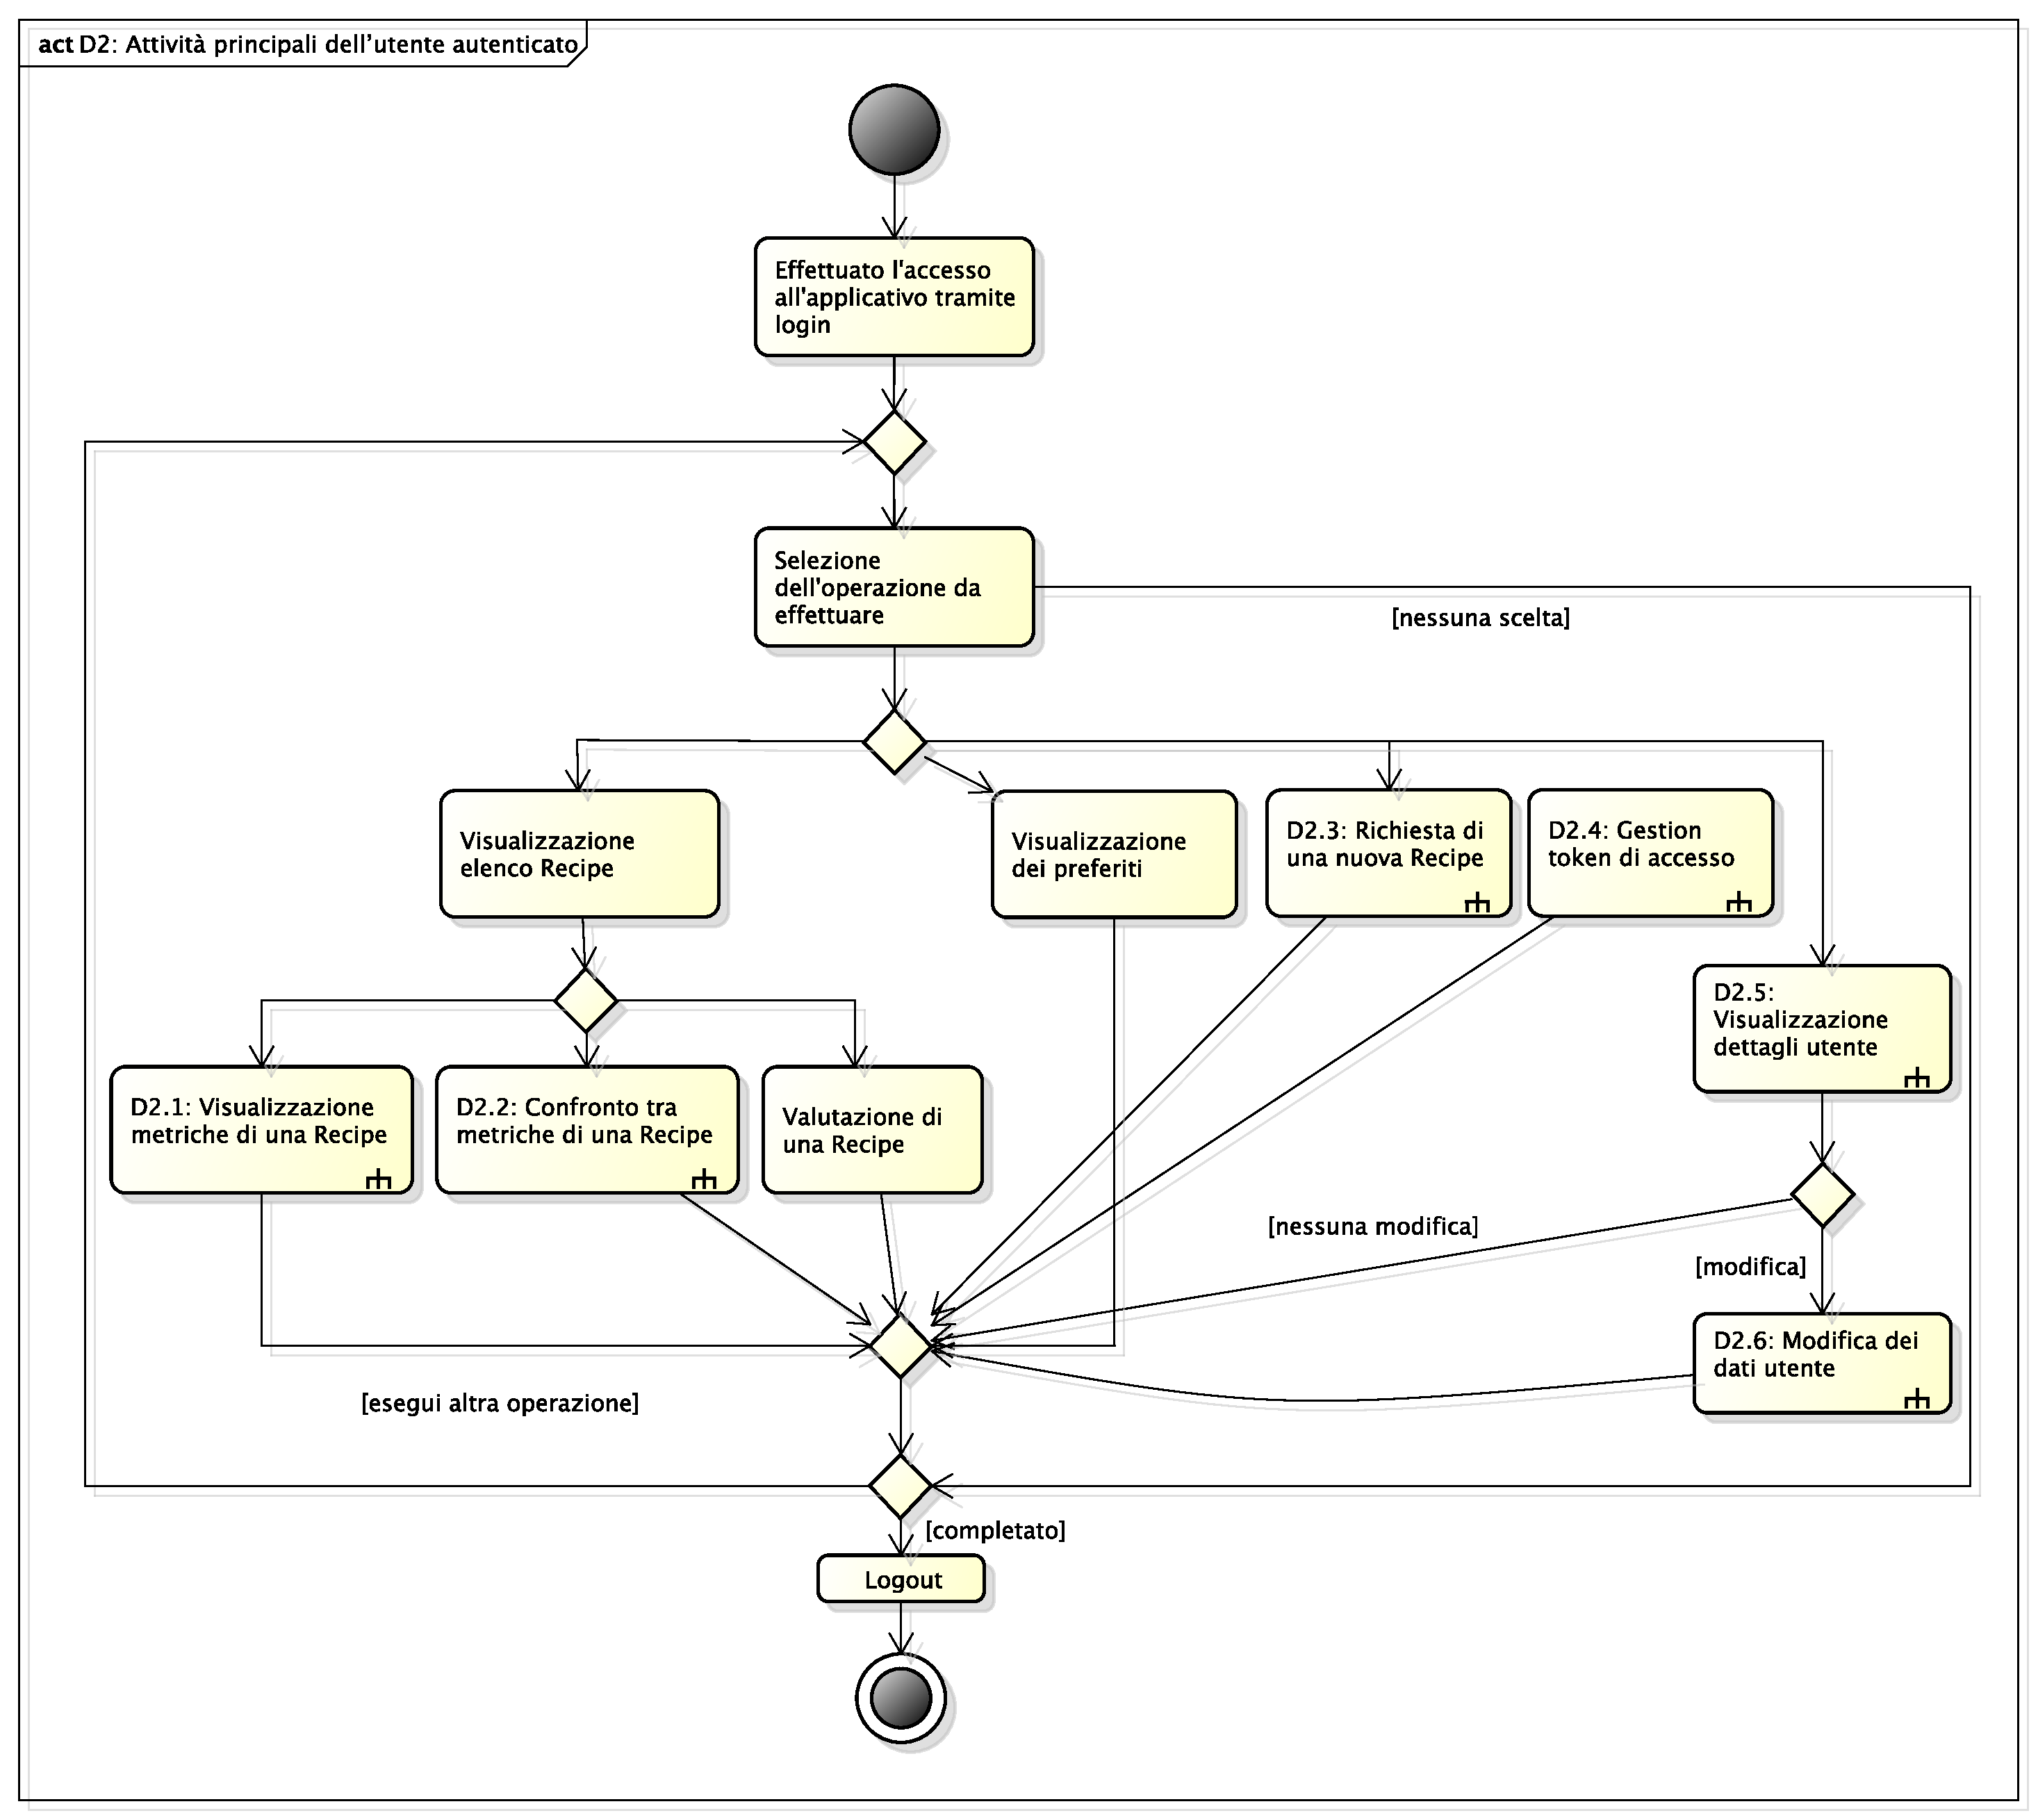
\includegraphics[scale=0.70]{./images/D2.pdf}}
			\caption{D2 - Diagramma delle attività principali dell'utente autenticato}
		\end{figure}
		\noindent
		Una volta effettuato l'accesso al sistema, l'utente ha la possibilità di compiere diverse azioni:
			\begin{itemize}
				\item Visualizzare l'elenco delle Recipe presenti nel sistema;
				\item Visualizzare le metriche di una Recipe particolare;
				\item Confrontare più metriche tra di loro;
				\item Valutare una Recipe;
				\item Visualizzare le View preferite;
				\item Richiedere l'inserimento di una nuova Recipe agli amministratori;
				\item Gestire il token d'accesso per utilizzare i servizi REST;
				\item Visualizzare e modificare i suoi dati personali.
			\end{itemize}
			\noindent
		Una volta conclusa l'operazione scelta, potrà eseguirne un'altra o effettuare il logout dal sistema.
		% subsubsection attività_principali_dell_utente_autenticato (end)


		\subsubsection{D2.1: Visualizzazione metriche di una Recipe} % (fold)
		\label{ssub:visualizzazione_metriche_di_una_recipe}
		\label{ssub:registrazione_al_sistema}
		\begin{figure}[!htbp]
			\centering
			\centerline{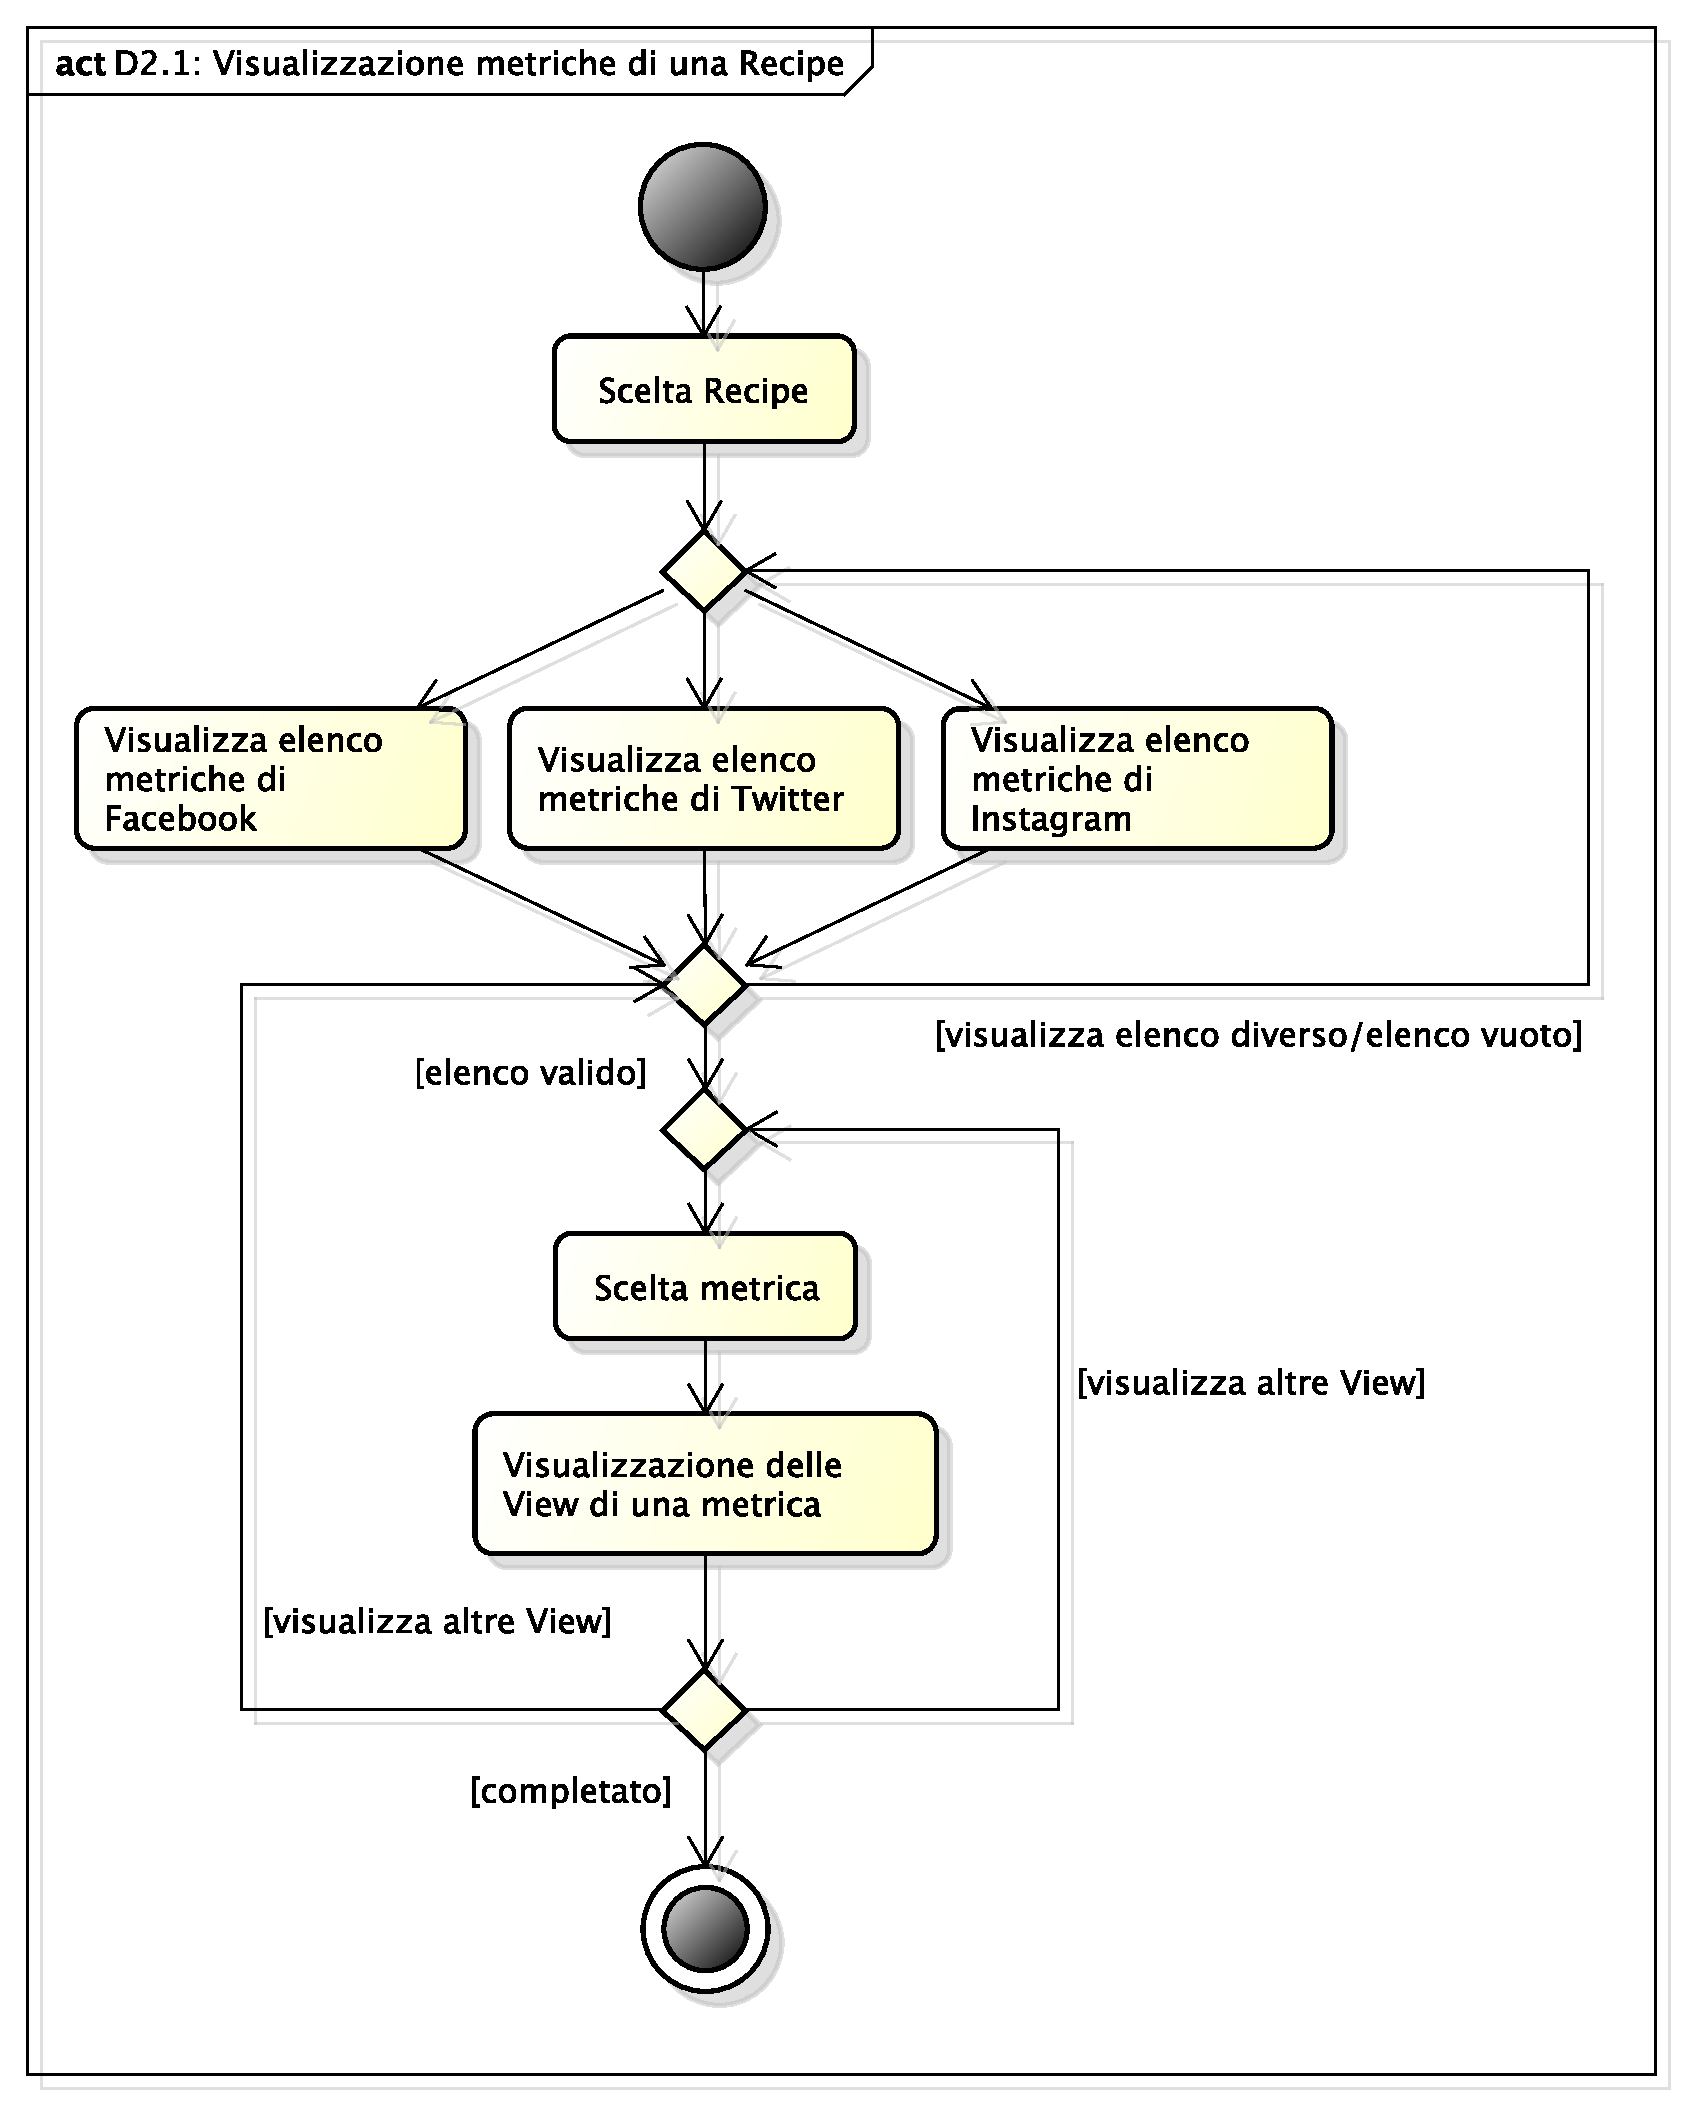
\includegraphics[scale=0.45]{./images/D2_1.pdf}}
			\caption{D2.1 - Diagramma della visualizzazione metriche di una Recipe}
		\end{figure}
		\noindent
		Dopo avere selezionato la Recipe, della quale si vuole vedere la lista delle metriche associate a essa, l'utente deve scegliere la categoria di appartenenza di queste metriche. Dovrà scegliere tra Facebook, Twitter o Instagram. Una volta deciso, comparirà una lista di tutte le metriche per quella categoria. Se l'utente desidera visualizzare le View generate da una metrica in particolare dovrà accedere a essa, altrimenti potrà cambiare categoria o concludere questa operazione.
		% subsubsection visualizzazione_metriche_di_una_recipe (end)


		\subsubsection{D2.2: Confronto tra metriche di una Recipe} % (fold)
		\label{ssub:confronto_tra_metriche_di_una_recipe}
		\begin{figure}[!htbp]
			\centering
			\centerline{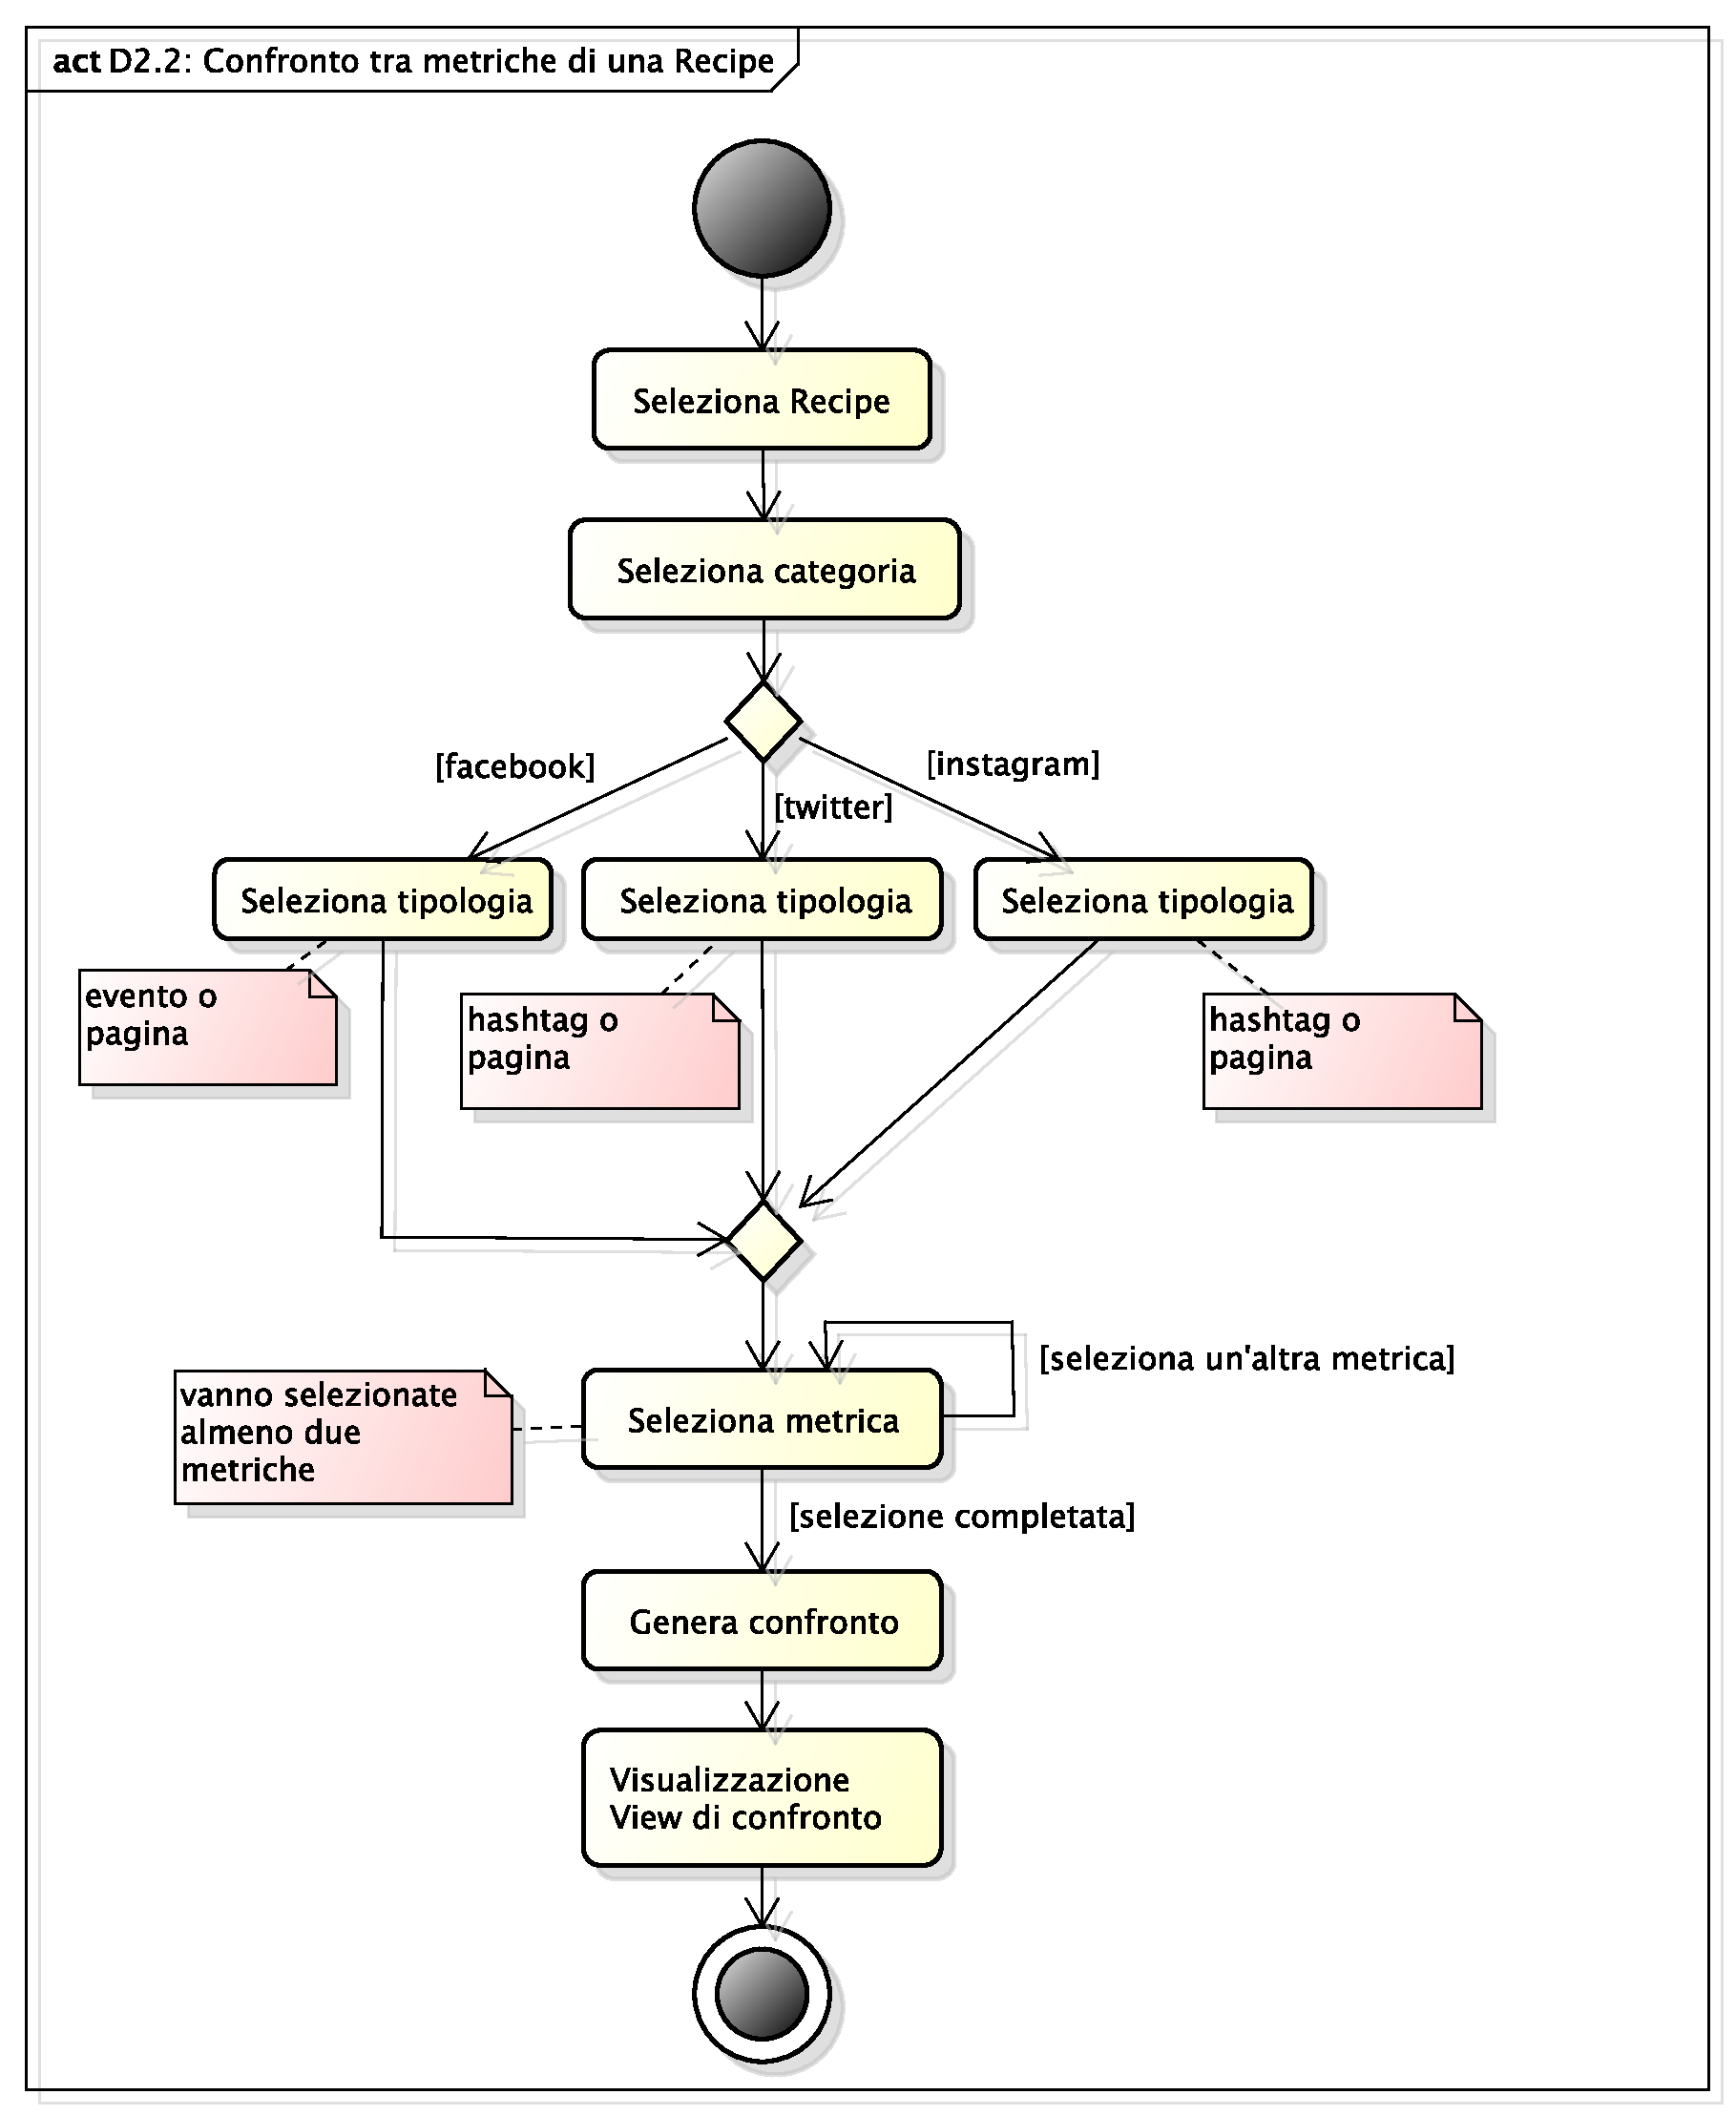
\includegraphics[scale=0.69]{./images/D2_2.pdf}}
			\caption{D2.2 - Diagramma del confronto tra metriche di una Recipe}
			\label{fig:d2_2}
		\end{figure}
		\noindent
		Dopo avere selezionato la Recipe, della quale si vuole utilizzare le metriche per generare dei confronti. L'utente deve seguire passo passo le scelte descritte nel diagramma \ref{fig:d2_2}. Questo comporterà alla visualizzazione delle View relative al confronto tra i valori scelti.
		% subsubsection confronto_tra_metriche_di_una_recipe (end)


		\subsubsection{D2.3: Richiesta di una nuova Recipe} % (fold)
		\label{ssub:richiesta_di_una_nuova_recipe}
		\begin{figure}[!htbp]
			\centering
			\centerline{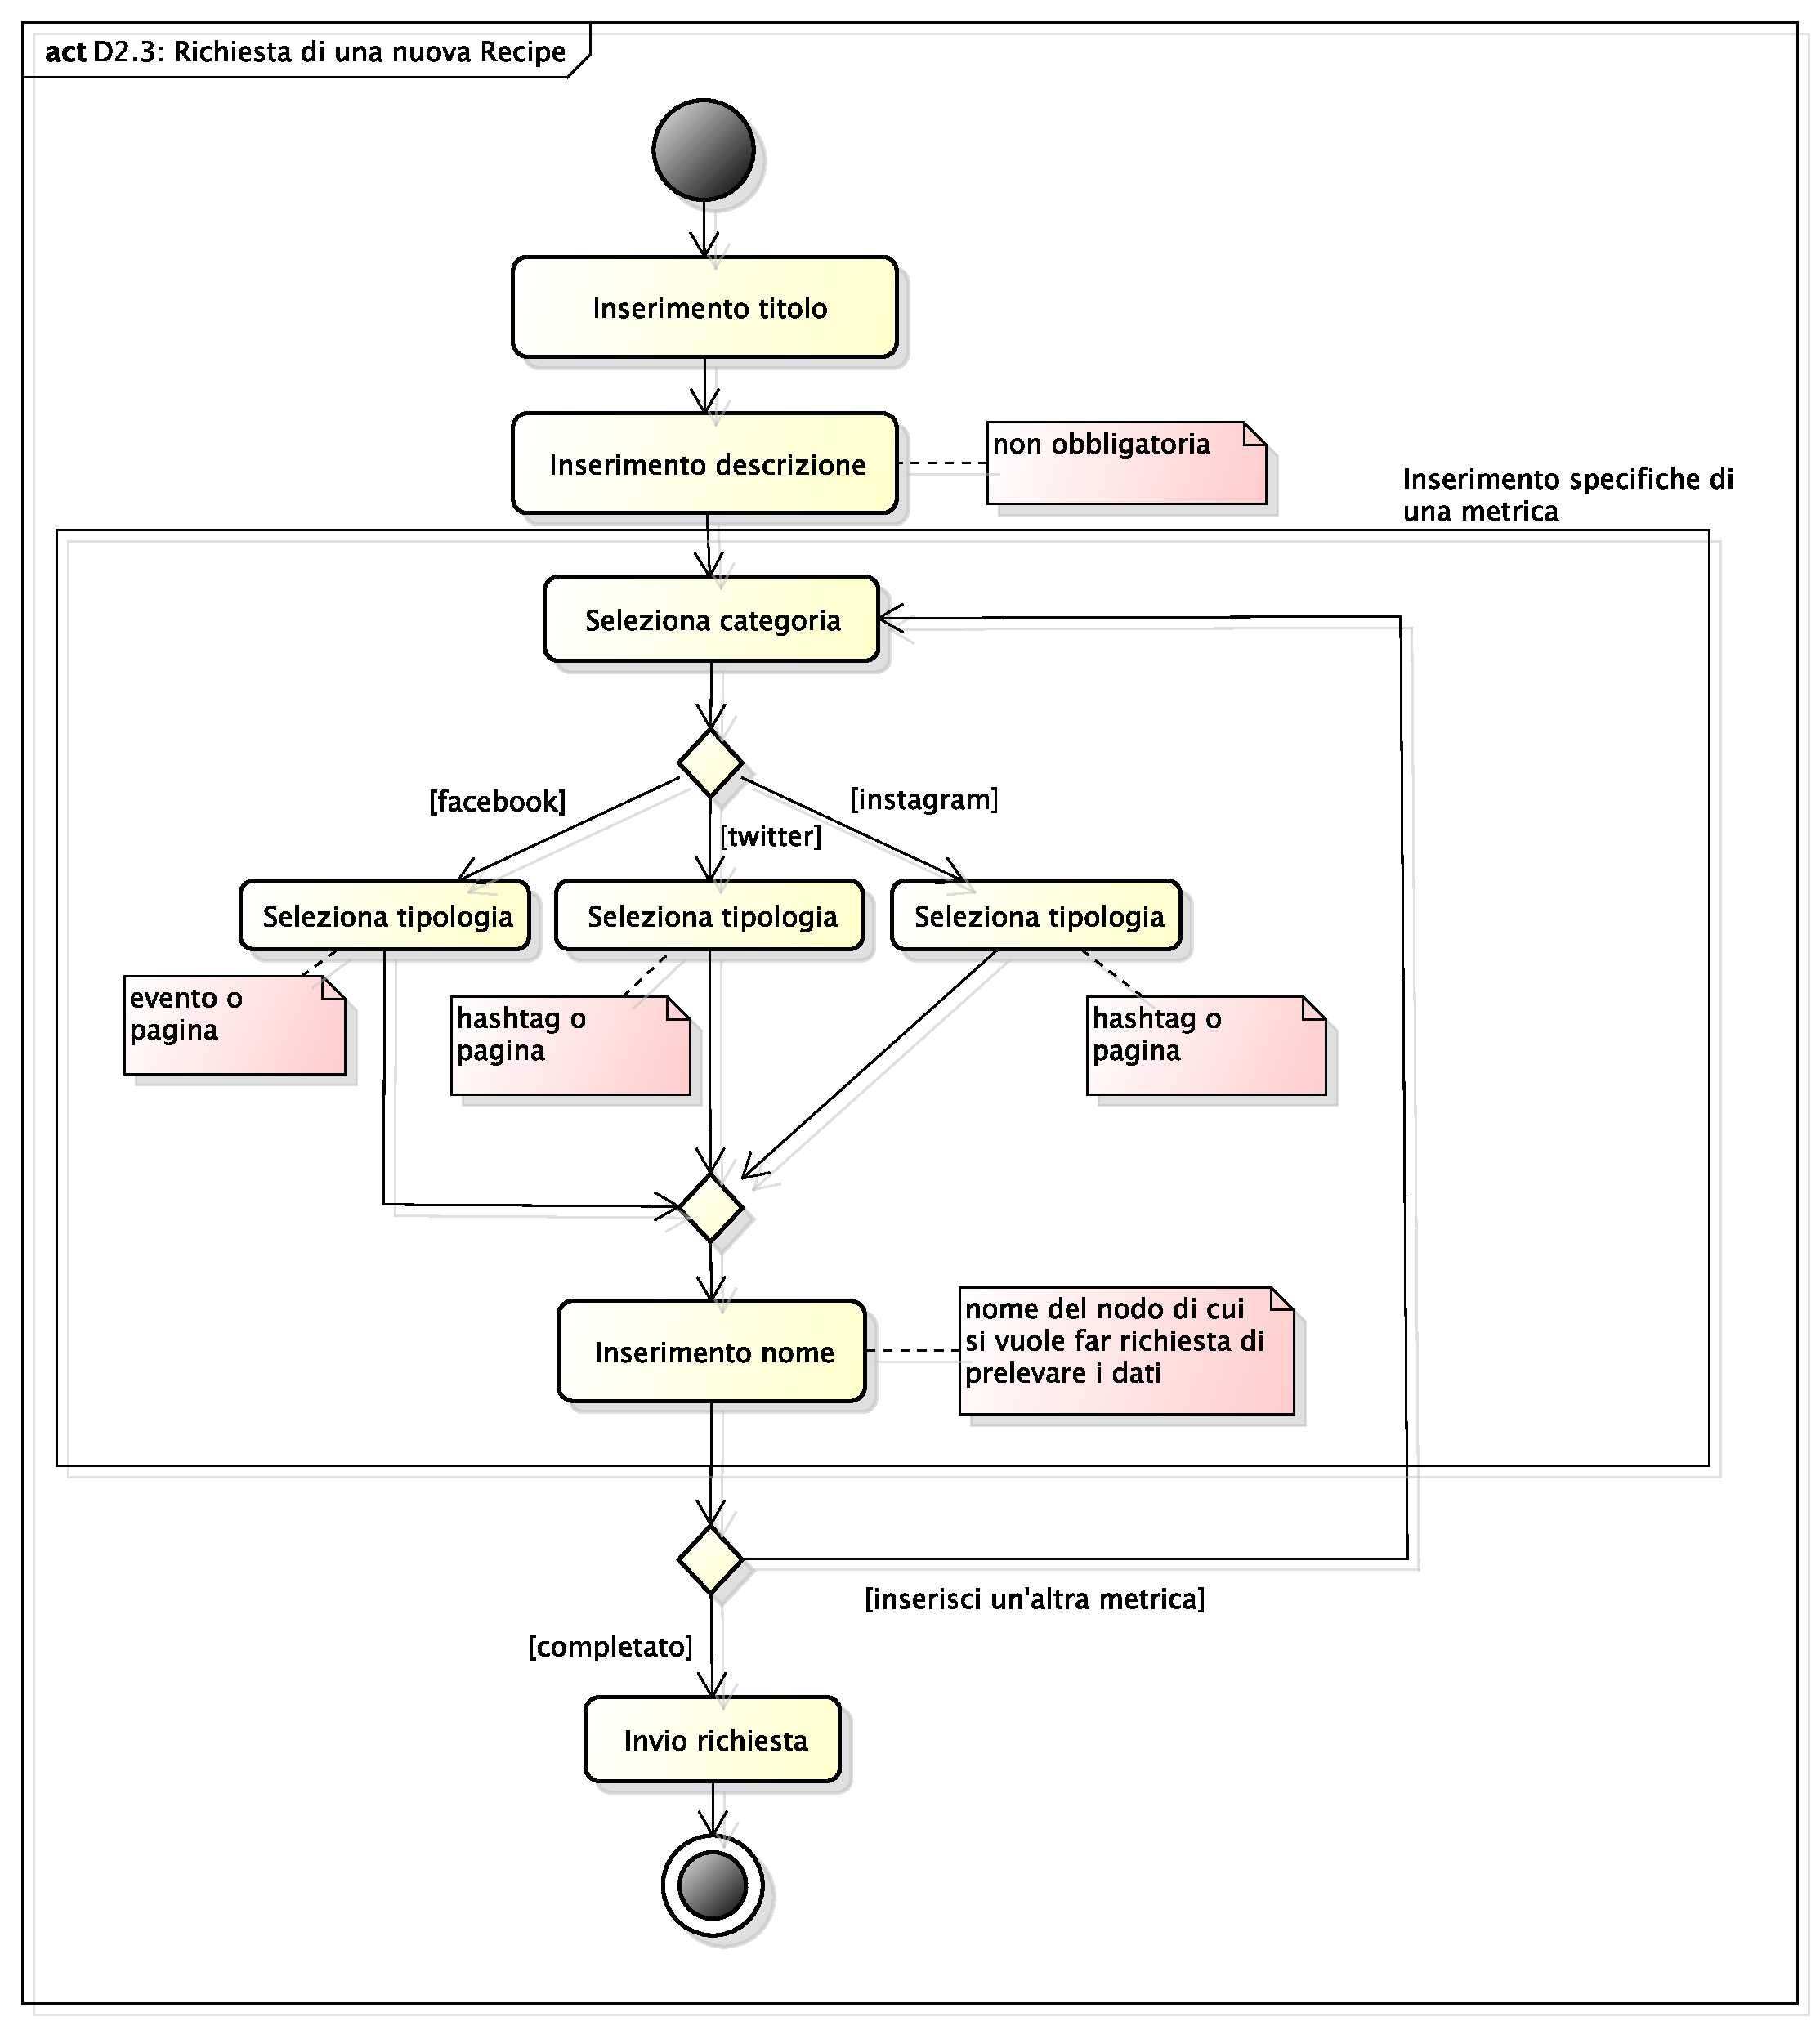
\includegraphics[scale=0.45]{./images/D2_3.pdf}}
			\caption{D2.3 - Diagramma della richiesta di una nuova Recipe}
		\end{figure}
		\noindent
		L'utente ha l'opportunità di fare delle richieste di inserimento di nuove Recipe nel sistema. Esso dovrà completare un form molto vincolato dal sistema, in modo che tutte le richieste seguano un determinato stile. Una volta completato, l'utente procederà all'invio della richiesta, la quale passerà agli amministratore che la valuteranno per approvarla o meno.
		% subsubsection richiesta_di_una_nuova_recipe (end)

		\subsubsection{D2.4: Gestione token di accesso} % (fold)
		\label{ssub:gestione_token_di_accesso}
		\begin{figure}[!htbp]
			\centering
			\centerline{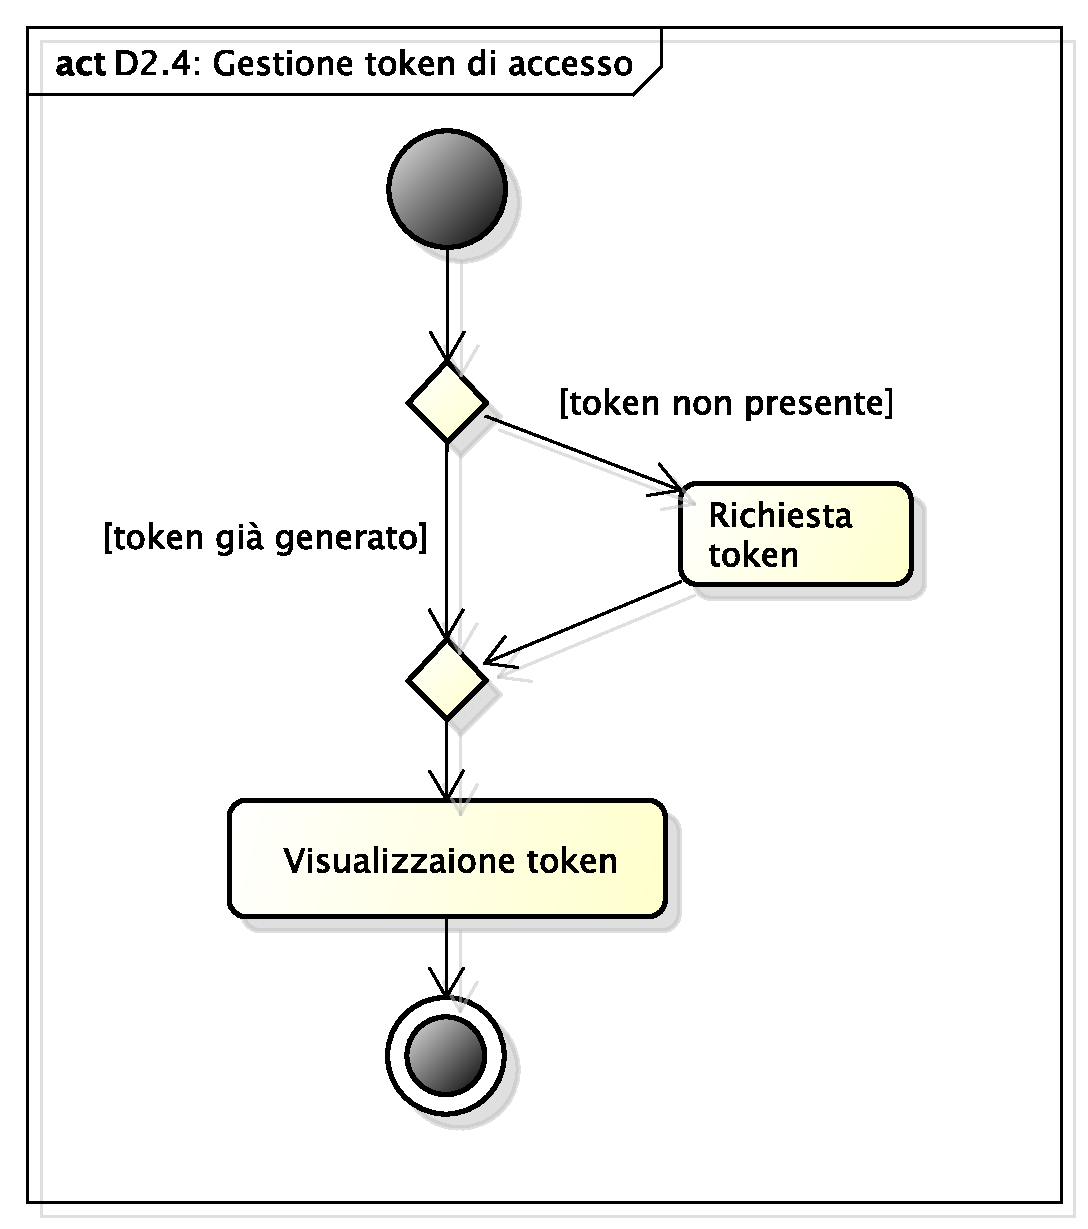
\includegraphics[scale=0.45]{./images/D2_4.pdf}}
			\caption{D2.4 - Diagramma della gestione del token di accesso}
		\end{figure}
		\noindent
		L'utente che si è registrato, al sistema, qualora fosse uno sviluppatore, potrà utilizzare i servizi REST che il sistema offre per utilizzare i dati nella maniera più utile al suo scopo. Per farlo dovrà richiedere un token di accesso che gli sarà fornito premendo su un apposito pulsante.
		% subsubsection gestione_token_di_accesso (end)

		\subsubsection{D2.5: Visualizzazione dettagli utente} % (fold)
		\label{ssub:visualizzazione_dettagli_utente}
		\begin{figure}[!htbp]
			\centering
			\centerline{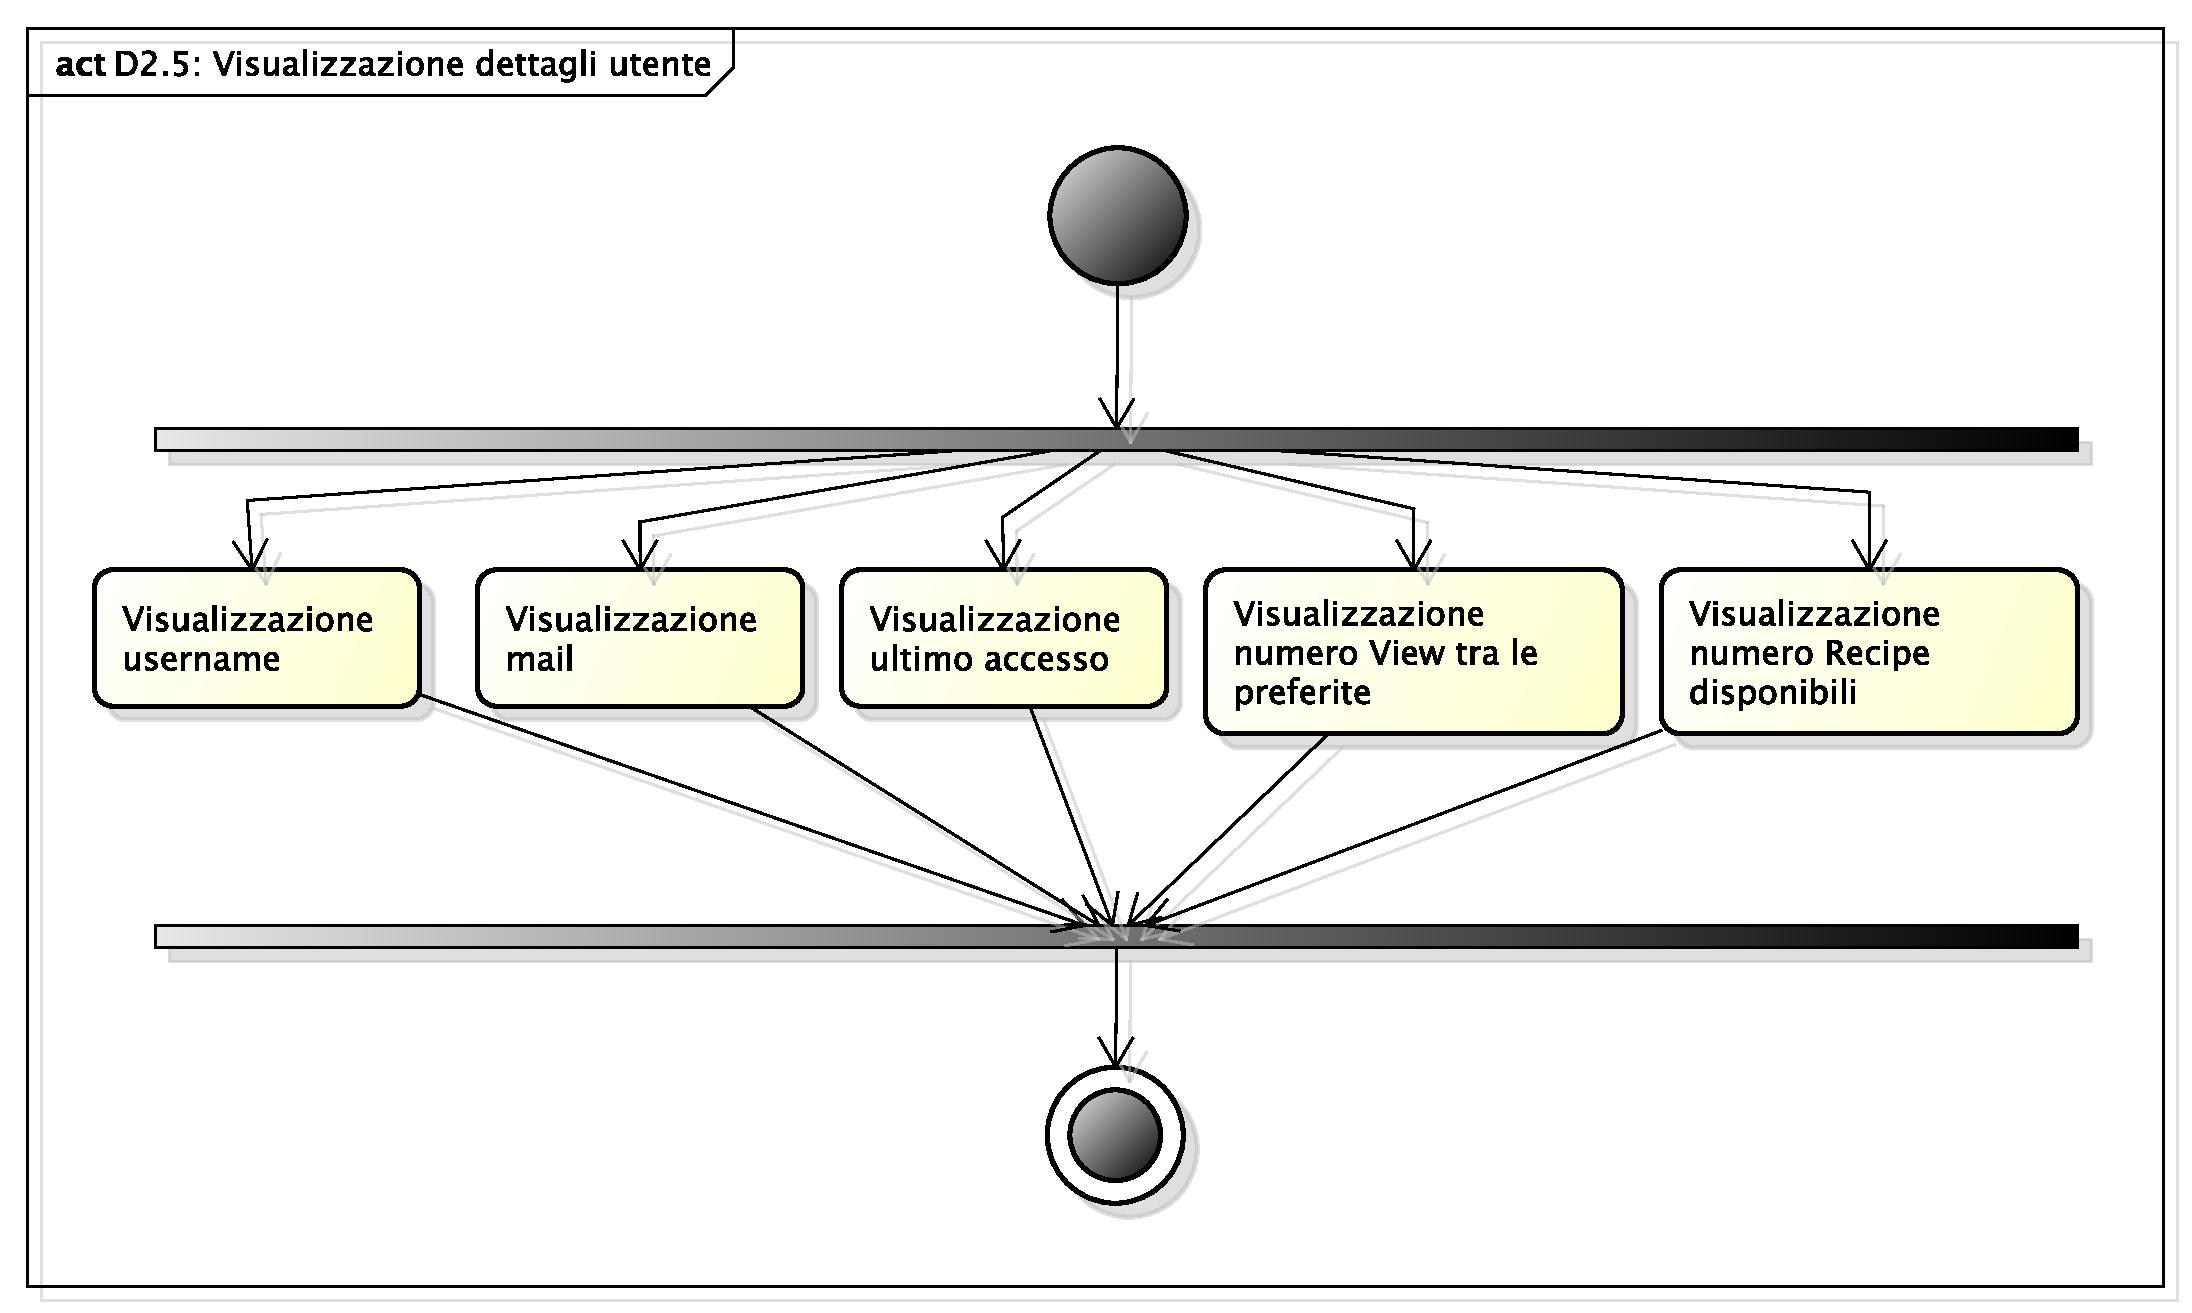
\includegraphics[scale=0.45]{./images/D2_5.pdf}}
			\caption{D2.5 - Diagramma della visualizzazione dettagli utente}
		\end{figure}
		\noindent
		L'utente potrà visualizzare in parallelo una serie di informazioni riguardanti il suo profilo.
		% subsubsection visualizzazione_dettagli_utente (end)

		\subsubsection{D2.6: Modifica dei dati utente} % (fold)
		\label{ssub:modifica_dei_dati_utente}
		\begin{figure}[!htbp]
			\centering
			\centerline{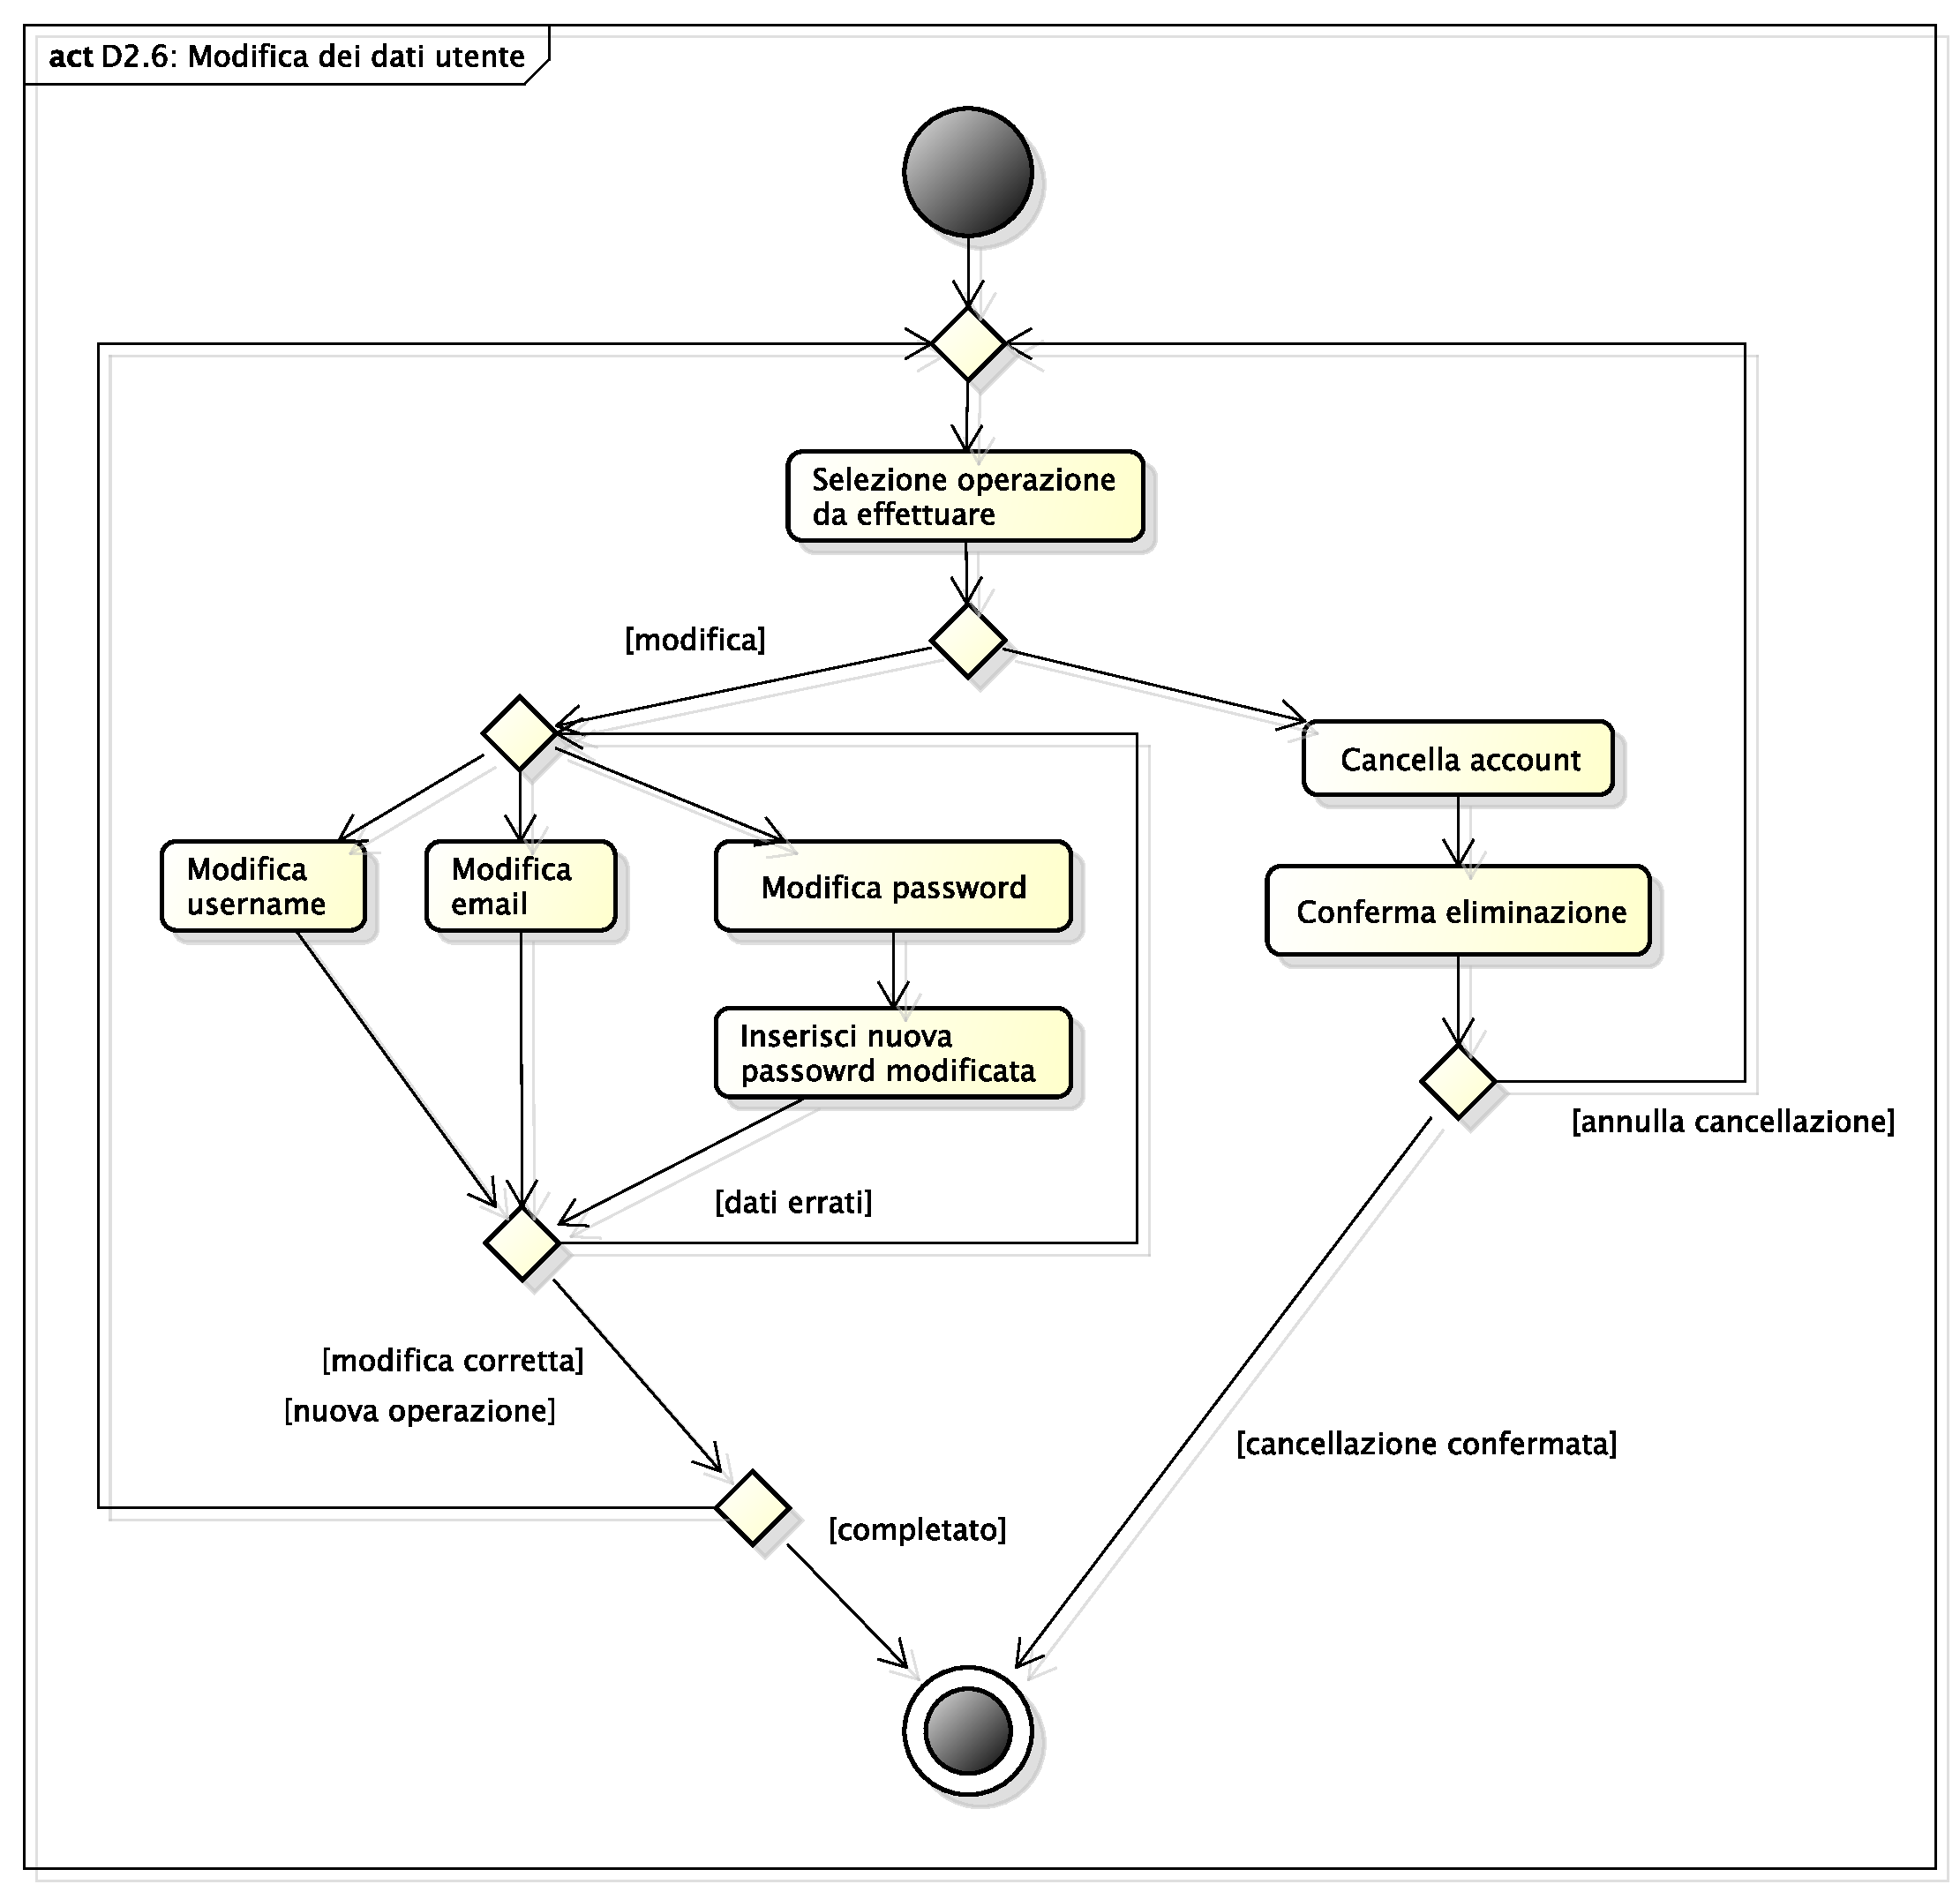
\includegraphics[scale=0.45]{./images/D2_6.pdf}}
			\caption{D2.6 - Diagramma della modifica dei dati utente}
		\end{figure}
		\noindent
		Oltre a visualizzare i dati associati al suo profilo, l'utente ne potrà modificare alcuni come lo username, l'email o la password. Potrà anche decidere di cancellarsi dall'applicazione andando ad eliminare l'account.
		% subsubsection modifica_dei_dati_utente (end)


	% subsection utente_autenticato (end)

	\pagebreak
	\clearpage \newpage


	\subsection{Utente amministratore} % (fold)
	\label{sub:utente_amministratore}
	In questa sezione vengono illustrate le attività che un amministratore del sistema può compiere. L'utente amministratore oltre alle suddette potrà svolgere anche tutte le attività presenti nella sezione \ref{ssub:attivita_principali_dell_utente_autenticato}.
		\subsubsection{D3: Attività principali dell'utente amministratore} % (fold)
		\label{ssub:attivita_principali_dell_utente_amministratore}
		\begin{figure}[!htbp]
			\centering
			\centerline{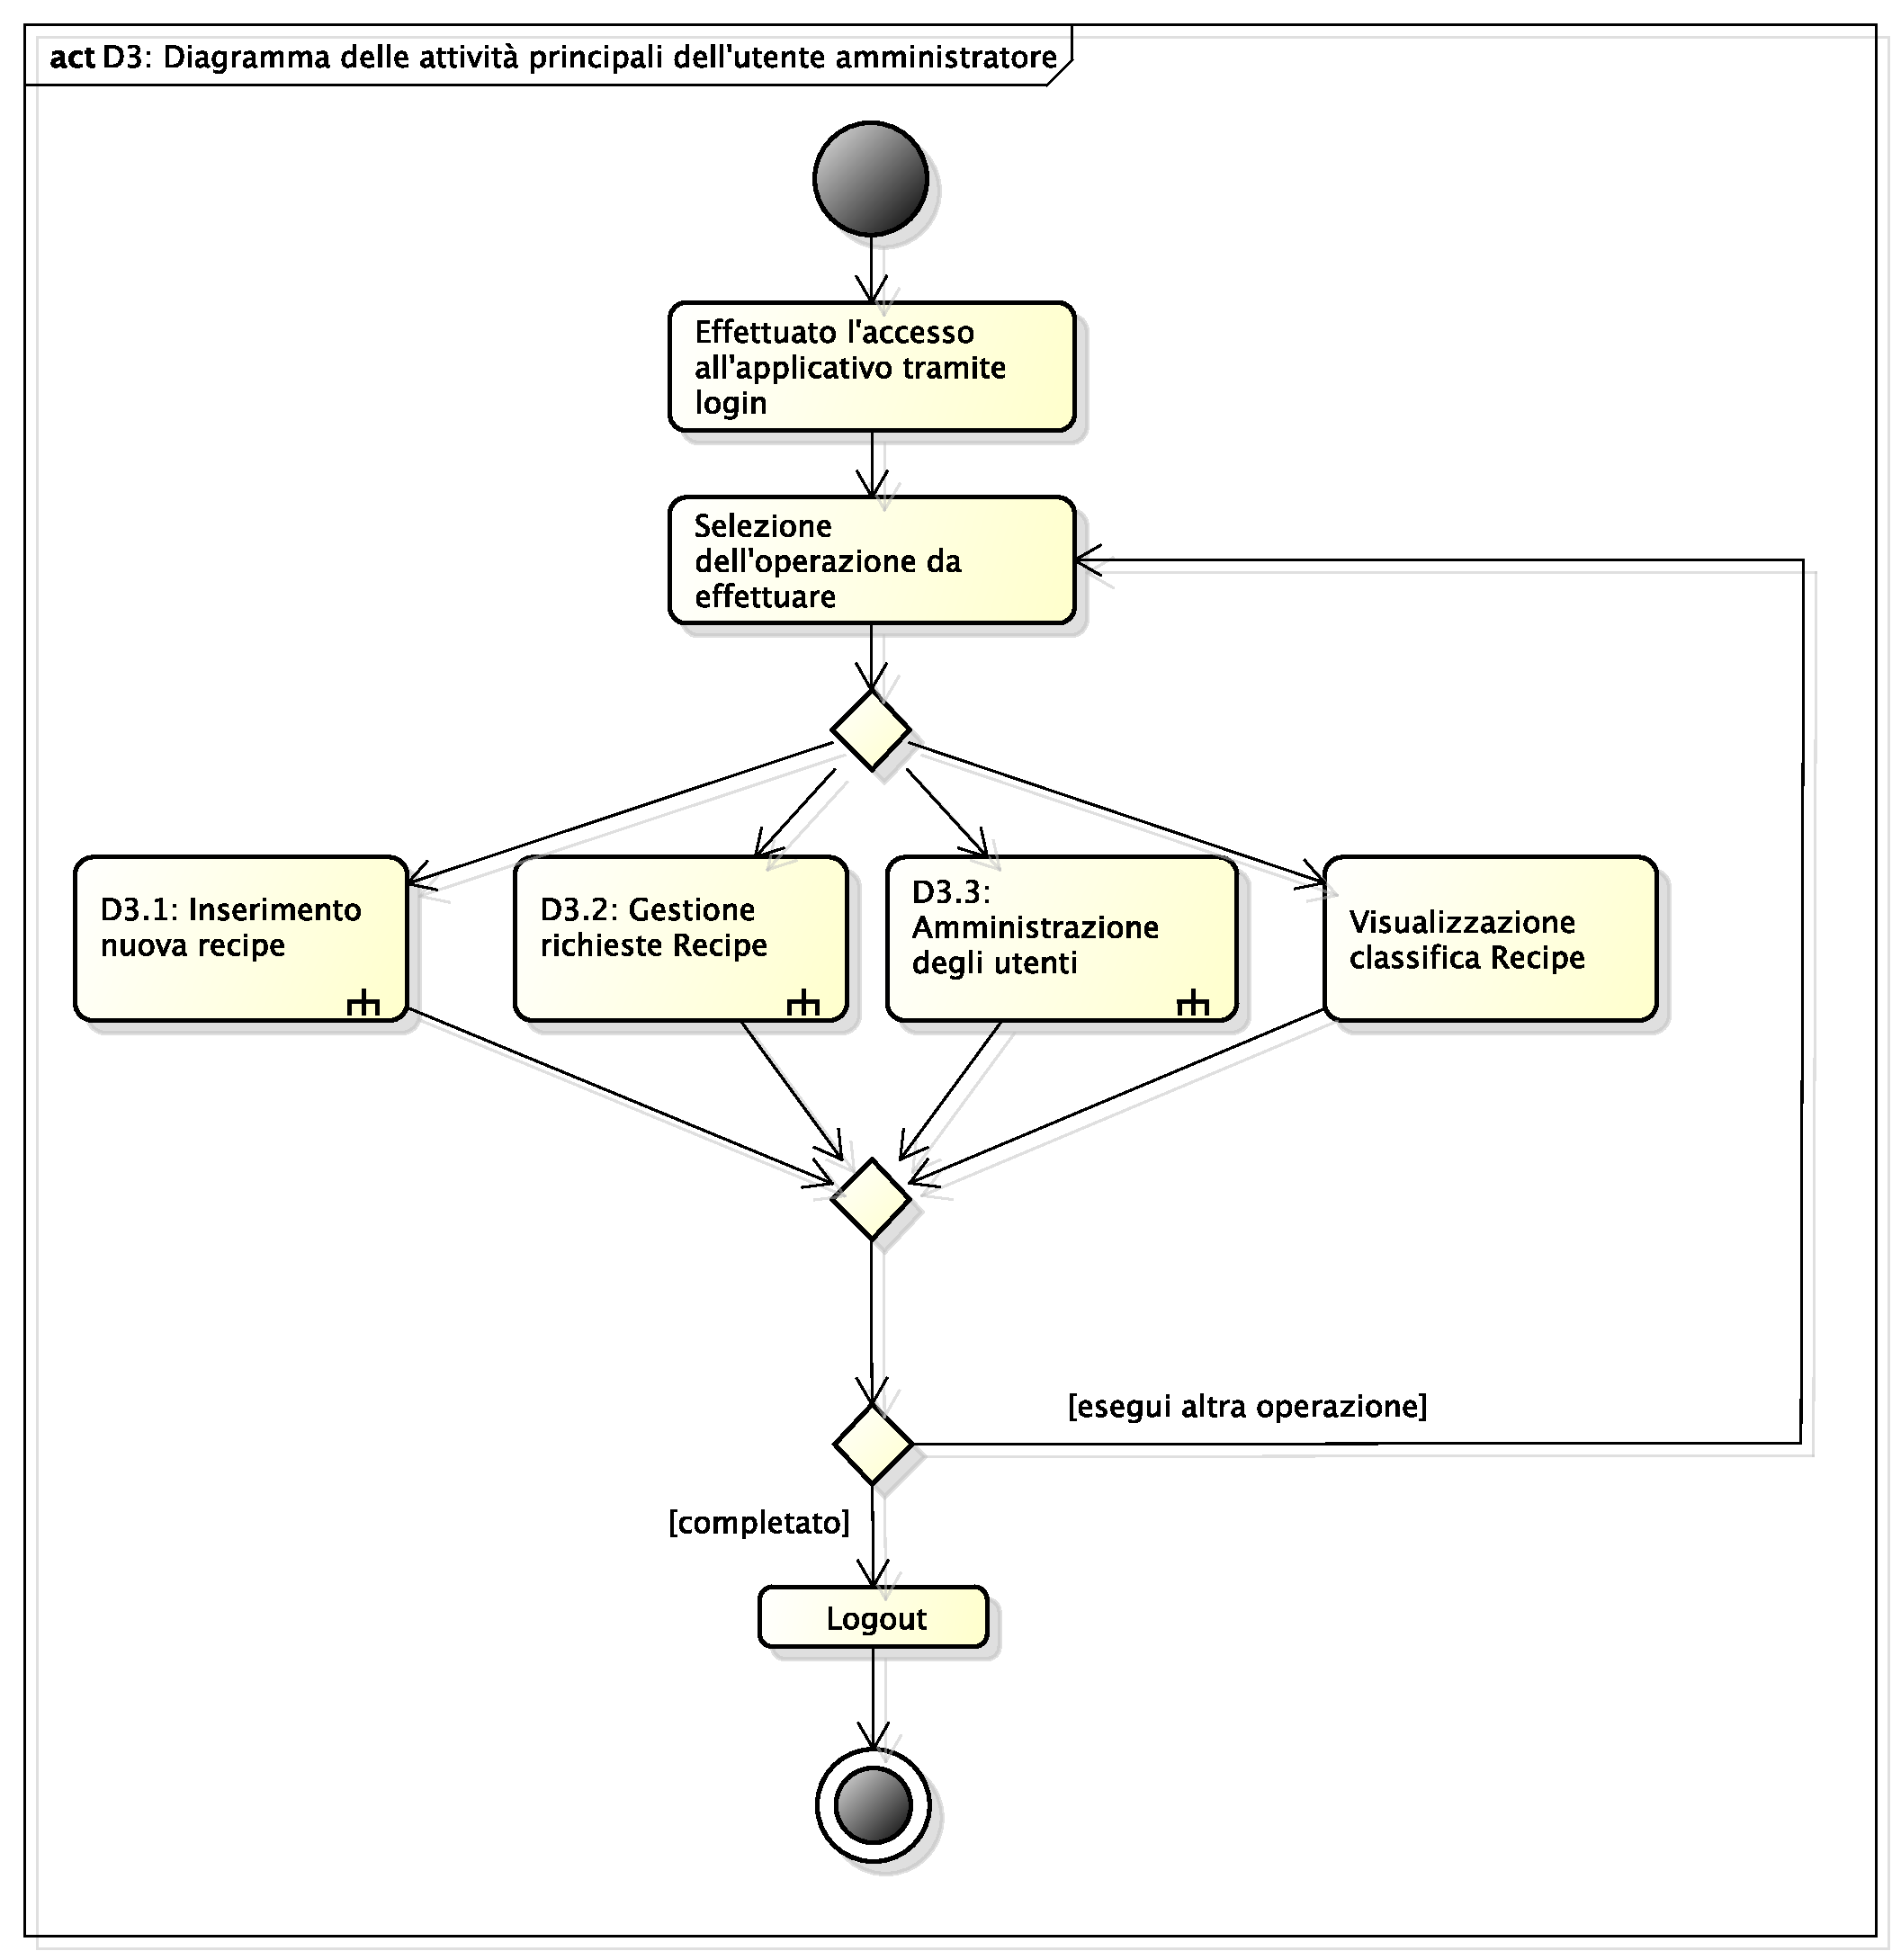
\includegraphics[scale=0.45]{./images/D3.pdf}}
			\caption{D3 - Diagramma delle attività principali dell'utente amministratore}
		\end{figure}
		\noindent
		Una volta effettuato l'accesso al sistema, l'amministratore ha la possibilità di compiere diverse azioni:
			\begin{itemize}
				\item Inserire nuova Recipe nel sistema;
				\item Gestire le richieste di nuove Recipe da parte degli utenti;
				\item Amministrare gli utenti;
				\item Visualizzare la classifica delle Recipe più apprezzate.
			\end{itemize}
			\noindent
		Una volta conclusa l'operazione scelta, potrà eseguirne un'altra o effettuare il logout dal sistema.

		% subsubsection attività_principali_dell_utente_amministratore (end)


		\subsubsection{D3.1: Inserimento nuova Recipe} % (fold)
		\label{ssub:inserimento_nuova_recipe}
		\begin{figure}[!htbp]
			\centering
			\centerline{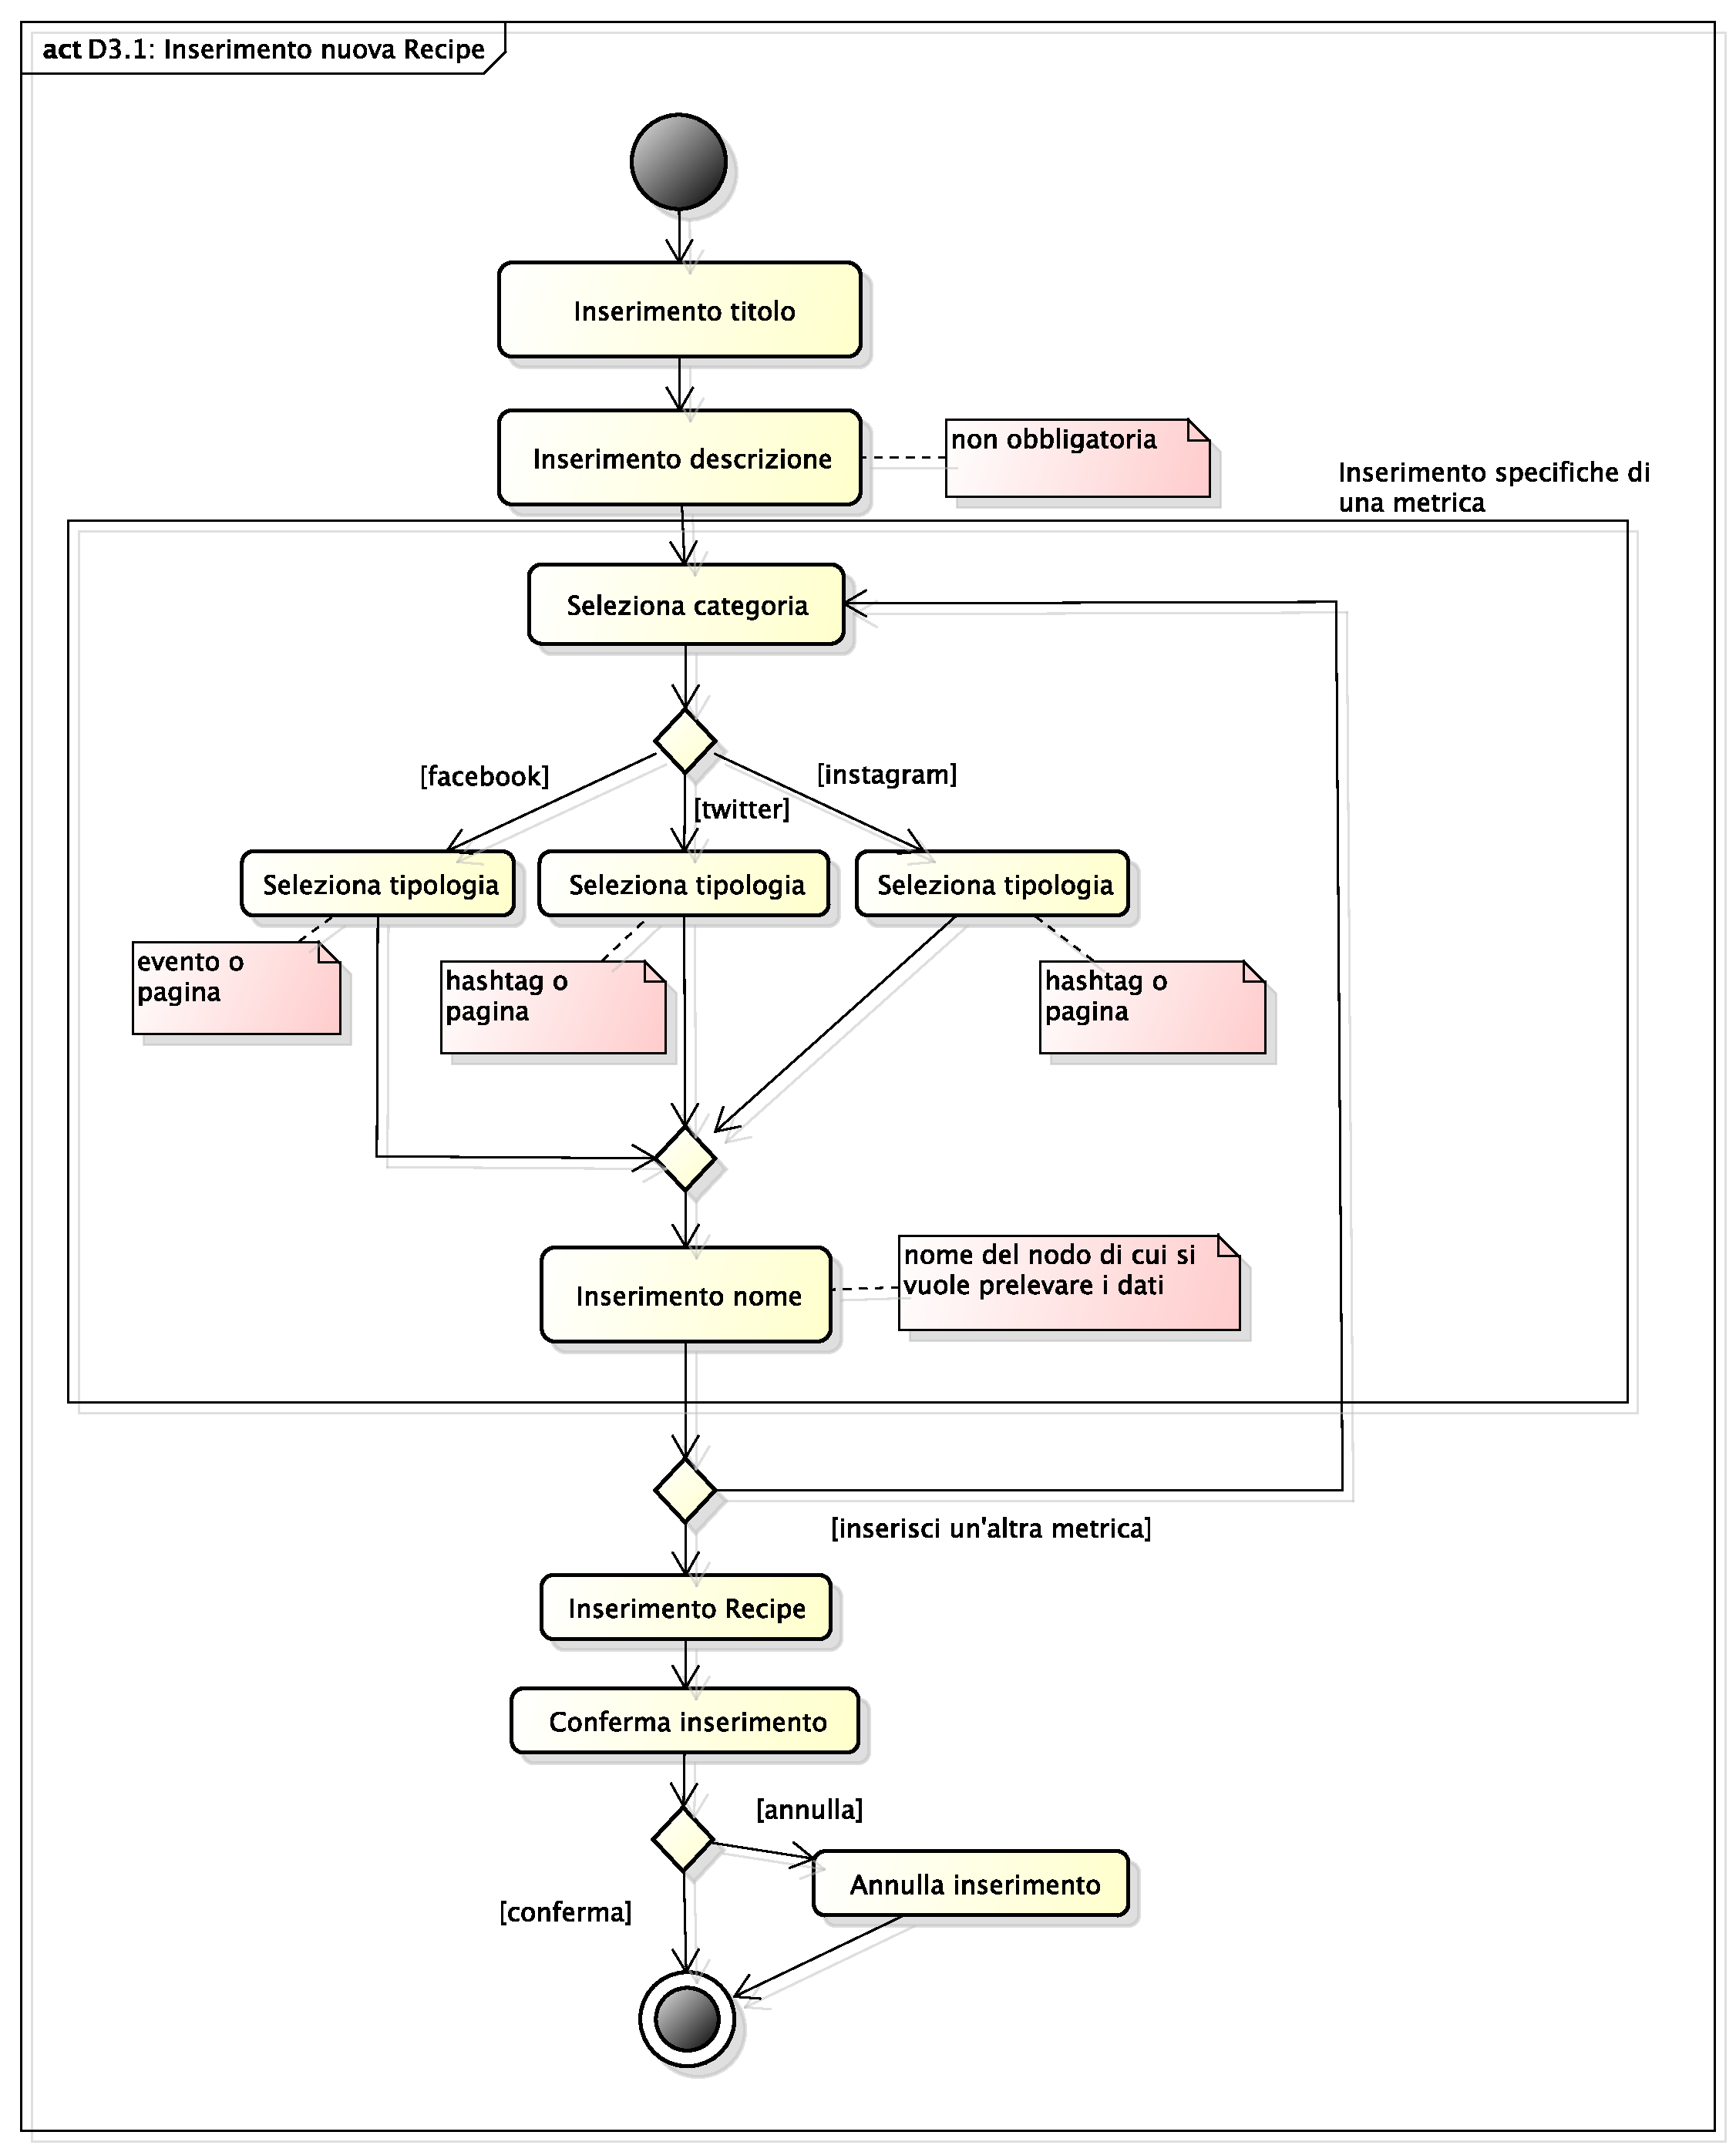
\includegraphics[scale=0.45]{./images/D3_1.pdf}}
			\caption{D3.1 - Diagramma dell'inserimento di una nuova Recipe}
		\end{figure}
		\noindent
		L'utente amministratore può decidere di inserire nuove Recipe nel sistema. Qualora volesse farlo, dovrà inserire una serie di dati richiesti da una form. Una volta completati i campi e verificata la correttezza da parte del sistema di essi, la Recipe verrà inserita nel sistema.
		% subsubsection inserimento_nuova_recipe (end)

		\pagebreak
		% \clearpage \newpage

		\subsubsection{D3.2: Gestione richieste Recipe} % (fold)
		\label{ssub:gestione_richieste_recipe}
		\begin{figure}[!htbp]
			\centering
			\centerline{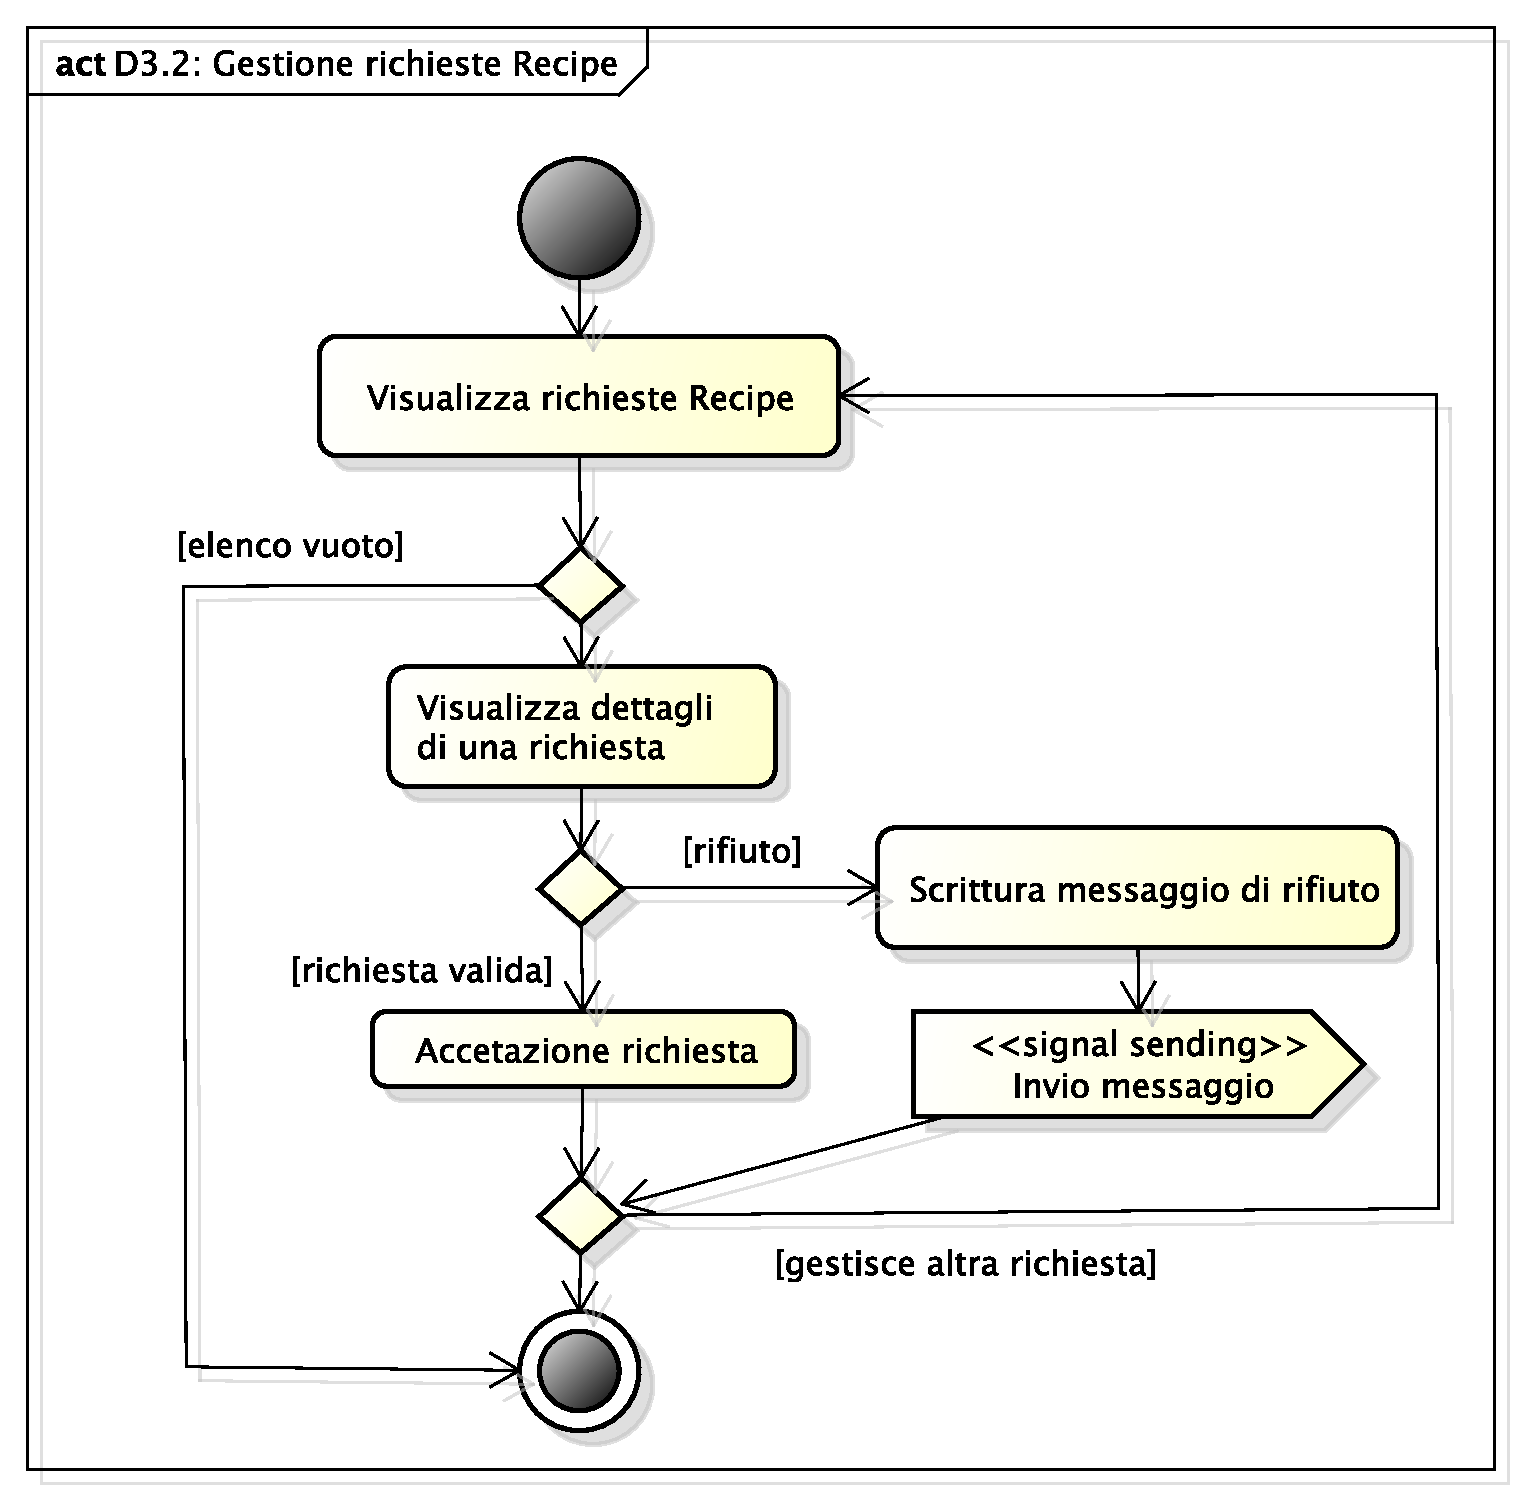
\includegraphics[scale=0.45]{./images/D3_2.pdf}}
			\caption{D3.2 - Diagramma della gestione delle richieste Recipe}
		\end{figure}
		\noindent
		L'amministratore ha il compito di valutare le richieste di nuove Recipe che gli vengono inviate dagli utenti. Visualizzerà quindi una form già riempita dei campi necessari ad generare la Recipe. I campi, saranno già corretti. All'amministratore è fornita solo la possibilità di modificare il titolo e la descrizione della Recipe, in modo da renderle più precise e significative anche per altri utenti, qualora la richiesta fosse accettata. \newline
		Se, però l'amministratore, si rende conto che la richiesta è troppo vaga e su argomenti scorrelati, potrò rifiutarla inviando un messaggio motivato al richiedente.
		% subsubsection gestione_richieste_recipe (end)

		\pagebreak

		\subsubsection{D3.3: Amministrazione degli utenti} % (fold)
		\label{ssub:amministrazione_degli_utenti}
		\begin{figure}[!htbp]
			\centering
			\centerline{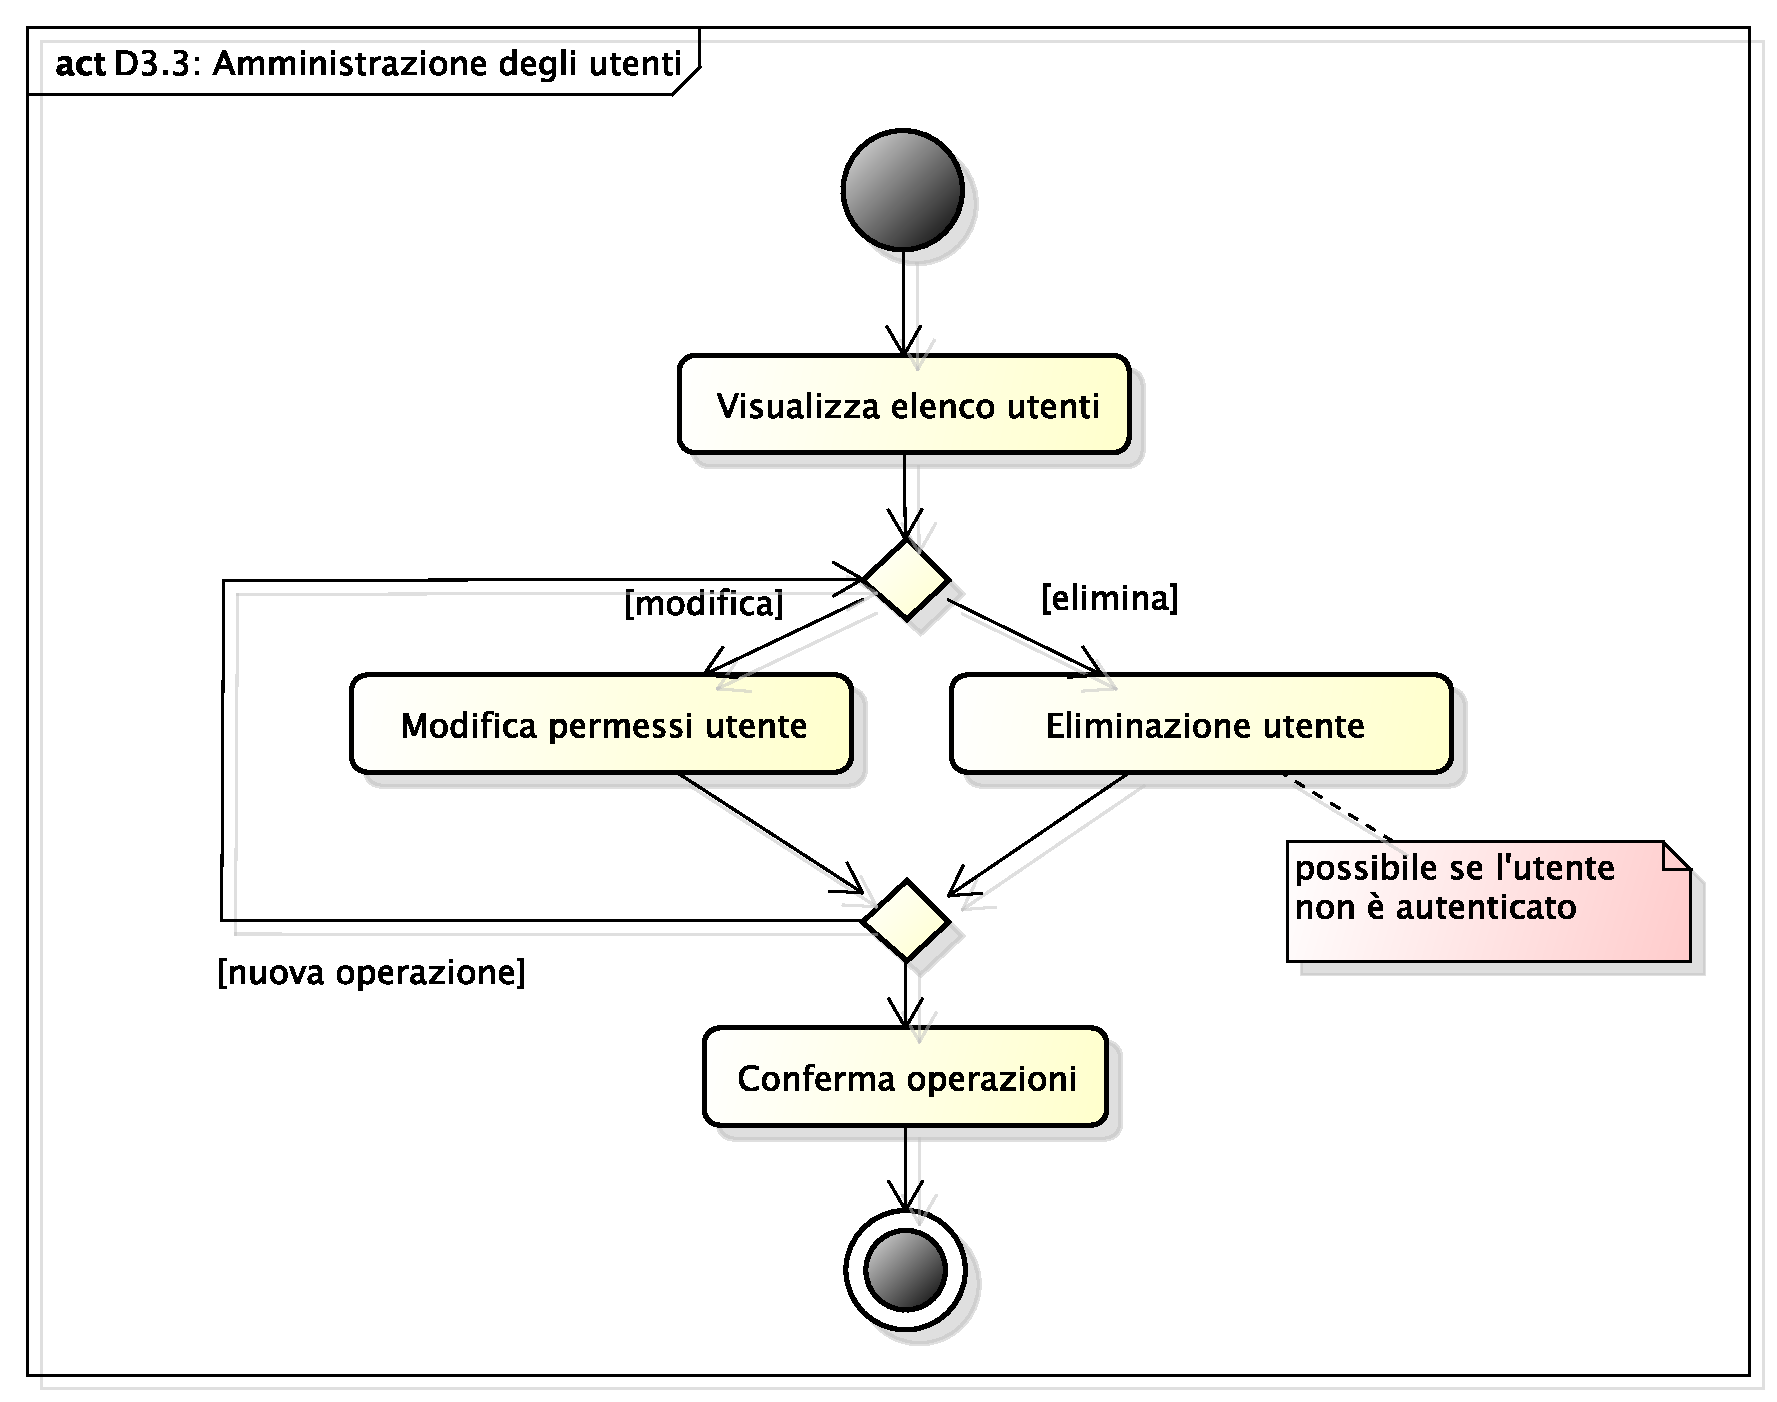
\includegraphics[scale=0.45]{./images/D3_3.pdf}}
			\caption{D3.3 - Diagramma dell'amministrazione degli utenti}
		\end{figure}
		\noindent
		All'amministratore è fornita anche la possibilità di modificare i permessi di un utente o di rimuoverlo dal sistema. L'eliminazione non potrà avvenire finché l'utente è dentro al sistema.
		% subsubsection amministrazione_degli_utenti (end)



	% subsection utente_amministratore (end)


% section diagrammi_delle_attività (end)